\documentclass[singlespacing, oneside]{unswthesis}

% Enables fixmes
\newif \ifDraft         \Draftfalse


% Status of the paper:
\Drafttrue
%\Draftfalse
%\Finaltrue

%\ifFinal\Draftfalse\fi

\ifDraft
  \usepackage{draftwatermark}
  \SetWatermarkLightness{0.85}
  \newcommand{\Comment}[1]{\textbf{\textsl{#1}}}
  \newenvironment{LongComment}[1] % multi-paragraph comment, argument is owner
    {\begingroup\par\noindent\slshape \textbf{\colorbox{yellow}{Begin Comment[#1]}}\par}
    {\par\noindent\textbf{\colorbox{yellow}{End Comment}}\endgroup\par}
  \newcommand{\FIXME}[1]{\textbf{\textsl{\colorbox{yellow}{FIXME:} #1}}}
  \newcommand{\TODO}[1]{\textbf{\textsl{\colorbox{yellow}{TODO:} #1}}}
\else
  \newcommand{\Comment}[1]{\relax}
  \newenvironment{LongComment}[1]{\expandafter\comment}{\expandafter\endcomment}
  \newcommand{\FIXME}[1]{\relax}
  \newcommand{\TODO}[1]{\relax}
\fi

\usepackage{graphicx}
\usepackage{listings}
\usepackage{courier}
\usepackage{cite}
\usepackage{pdflscape}
\usepackage{longtable}
\usepackage{caption}
\usepackage{subcaption}
\usepackage{multicol}
\usepackage{fancyvrb}
\usepackage{tcolorbox}
\usepackage{etoolbox}
\usepackage[outputdir=obj/]{minted}
\usepackage{hyperref}
\usepackage{tikz}
\usepgflibrary{shapes.arrows}

\BeforeBeginEnvironment{minted}{\begin{tcolorbox}}
\AfterEndEnvironment{minted}{\end{tcolorbox}}

\newif \ifhyperlinks    \hyperlinkstrue
%%% Class options:

%  undergrad (default)
%  hdr

%  11pt (default)
%  12pt

%  final (default)
%  draft

%  oneside (default for hdr)
%  twoside (default for undergrad)


%% Thesis details
\thesistitle{High-performance Networking-based Systems on seL4}
\thesisschool{School of Computer Science and Engineering}
\thesisauthor{Lucy Parker}
\thesisZid{z5059323}
\thesisdegree{Bachelor of Computer Science (Honours)}
\thesisdate{November 2023}
\thesissupervisor{Prof.\ Gernot Heiser \& Dr Peter Chubb}% for undergrad theses only
%\thesisproject{}
\graphicspath{{imgs/}{imgs/benchmarks/}}

%% My own LaTeX macros, definitions, etc
%%%% Shortcuts
\newcommand{\num}[2]{\mbox{#1\,#2}}			% num with units

%%%% Symbols
\newcommand{\yes}{\ensuremath{\surd}\xspace}		% Tick mark
\newcommand{\no}{\ensuremath{\times}\xspace}		% Cross mark
\newcommand{\by}{\ensuremath{\times}\xspace}		% XXX x XXX
\newcommand{\bAND}{\ensuremath{\wedge}\xspace}		% Bool. /\
\newcommand{\bOR}{\ensuremath{\vee}\xspace}		% Bool. \/
\newcommand{\becomes}{\ensuremath{\rightarrow}\xspace}	% -->

\newcommand{\fontsmall}{\fontsize{7pt}{8pt}\selectfont}
\newcommand{\fontnormal}{\fontsize{11pt}}

%%%% Custom environments

% Centered tabular with single spacing
\newenvironment{ctabular}[1]
    {\par\begin{sspacing}\begin{center}\begin{tabular}{#1}}%
    {\end{tabular}\end{center}\end{sspacing}}


%%%% Our default level for display in TOC - subsubsections
\setcounter{tocdepth}{3}
\setcounter{secnumdepth}{5}



\begin{document}

\renewcommand{\sectionautorefname}{Section}
\renewcommand{\chapterautorefname}{Chapter}
\renewcommand{\subsectionautorefname}{Section}
\renewcommand{\subsubsectionautorefname}{Section}
\renewcommand{\appendixautorefname}{Appendix}

%% pages in the ``frontmatter'' section have roman numeral page number
\frontmatter  
\maketitle
\chapter{Abstract}\label{ch:abstract}

Modern operating systems undergo rapid development on an extensive code base. 
This growth has steadily introduced bugs and security vulnerabilities into the trusted computing base,
and the growing array of security patches and new features has led to a decline in system call performance.
Unfortunately, monolithic kernel design means a single exploitable vulnerability can compromise the entire kernel.
The alternative in microkernel-based design has historically been unpopular due to its impact on performance
as it requires significantly more context switches than its monolithic counterpart. This thesis evaluates the
seL4 Device Driver Framework which rectifies this concern, showcasing superior networking performance
compared to a standard Linux system, while leveraging the security guarantees
of the seL4 microkernel to provide a secure and performant networking subsystem. We extend the framework
to flexibly and securely support multiple client applications and scale to multi-core systems, 
highlighting a number of ways in which system designers can enforce use-case specific policies. 

\chapter*{Abbreviations}\label{abbr}
\begin{description}
\item[ARP] Address Resolution Protocol
\item[CC] Communication Channel
\item[CVE] Critical Vulnerabilities and Exposures
\item[DMA] Direct Memory Access
\item[FIFO] First In, First Out
\item[IDL] Interface Definition Language
\item[I/O] Input/Output
\item[IOMMU] Input, Output Memory Management Unit
\item[IoT] Internet of Things
\item[IP] Internet Protocol
\item[IPC]Inter-process Communication
\item[LOC] Lines of Code
\item[MAC] Media Access Control
\item[MPMC] Multi Producer, Multi Consumer
\item[MR] Memory Region
\item[MUX] Multiplexer
\item[NIC] Network Interface Controller
\item[OS] Operating System
\item[PD] Protection Domain
\item[PPC] Protected Procedure Call
\item[RPC] Remote Procedure Call
\item[Rx] Receive
\item[sDDF] The seL4 Device Driver Framework
\item[SPSC] Single Producer, Single Consumer
\item[TCB] Trusted Computing Base
\item[Tx] Transmit
\item[UDP] User Datagram Protocol
\end{description}


\tableofcontents
\listoffigures  % if required
% \listoftables  % if required

%% pages in the ``mainmatter'' section have arabic page numbers and chapters are numbered
\mainmatter

\chapter{Introduction}\label{ch:intro}

Typical networking-focused systems face major problems with either security, performance or both.
This thesis explores a novel I/O framework on seL4 for secure, high-performance
networking-based systems and extends the framework to support multi-client systems.

\section{The problem with I/O on monolithic kernels}
Operating systems are designed to abstract over hardware while
providing a consistent interface to applications. In a monolithic kernel
such as Linux, the kernel houses device drivers, file systems and network 
stacks. This means that these services run in privileged mode, and user 
applications make system calls in order to utilise these services and perform I/O.
However, there are two major problems with this design:
it is inherently insecure and historically, performs poorly.

\subsection{Monolithic kernels are fundamentally insecure}
Modern operating systems see a rapid development rate on a huge code base.
\autoref{f:growth} shows the exponential growth of the Linux kernel
(extracted from \cite{Linux:archives}) which sees over 70 thousand commits a year.
With this growth, bugs and security vulnerabilities are steadily brought into the 
trusted computing base.

\begin{figure}[h]
  \centering
  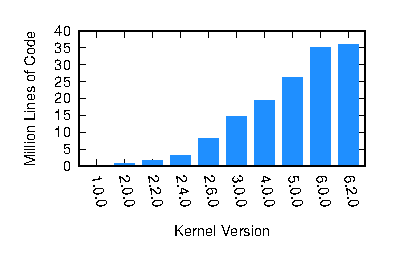
\includegraphics[width=10cm]{growth.eps}
  \caption{Growth of the Linux Kernel.}
  \label{f:growth}
\end{figure}

While much of this growth can be attributed to kernel extensions, such as drivers for new devices,
these extensions should not be overlooked. A modern Linux kernel runs around 80 - 130
device drivers on a given configuration \cite{Linux:LKDDB}, and drivers account for a significant
portion of critical vulnerabilities and exposures (CVE). \autoref{f:cves} shows the proportion of 
CVEs published in the last 5 years that can be attributed directly to drivers (extracted 
from \cite{Linux:CVEs}), with an average of 38\%.

\begin{figure}[h]
  \centering
  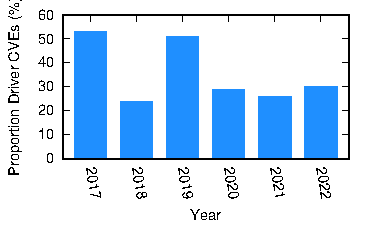
\includegraphics[width=10cm]{cves.pdf}
  \caption{Proportion of Linux CVEs due to device drivers.}
  \label{f:cves}
\end{figure}

The reason behind such a high rate of Linux CVEs is due largely to the fact that
drivers are typically written by hardware engineers as opposed to OS experts, and the growing
complexity of the kernel, has made kernel programming extremely difficult \cite{Swift_MLE_02}.\\
While modern kernels deploy a number of security mechanisms to protect their execution,
a large portion of vulnerabilities remains exploitable \cite{Narayanan_HTJB_20}. For example,
even advanced defence mechanisms, such as code pointer integrity (CPI) and safe stacks,
that protect the control flow of an application \cite{Kuznetsov_SPCSS_14}, remain
vulnerable to data-only attacks. These attacks, which focus on altering or forging
the critical data of an application can be combined with automated attack
generation tools to load disabled modules or manipulate attributes of pages in memory
\cite{Ispoglou_AJP_18}. Unfortunately, the monolithic design means a single exploitable
vulnerability potentially provides an attacker with access to the entire kernel.

\subsection{Performance limitations of monolithic kernels}
The monolithic design minimises the frequency of switching between kernel and user mode, enabling 
applications to trigger I/O with a single system call. However, the increasing number of security
enhancements and new features introduced to Linux has steadily added overhead to core
kernel operations and severely impacted system call performance. Ren et al. (2019) found
that the \emph{send()} and \emph{recv()} system calls, used to send and receive a packet over the
network, have slowed down by 100\% between Linux versions 4.0 and 4.2.
Furthermore, the monolithic design requires copying data between user and kernel space for I/O system
calls in order to sanitise the request and protect the kernel from a clumsy/malicious application. 
The cost of this data copying adds consistent overhead to such system calls and can quickly
become a bottleneck for high performance I/O systems.

\section{How do we rectify this?}
It's clear that we need to remove device drivers from the trusted computing base (TCB). However, simply 
running them as user level programs on a monolithic kernel requires careful design to prevent introducing
more costly system calls and further degrading performance. Such designs are already mainstream but unfortunately
are not without their own limitations. We explore these in \autoref{ch:related_work}. We examine how
asynchronous APIs can improve
performance in networking-based systems by reducing the system call overhead without addressing the security
implications of in-kernel drivers in \autoref{s:async}. In \autoref{s:userspace_dd}, we investigate I/O frameworks
that relegate all I/O processing, driver included, to user space. Such designs provide strong fault isolation to
drivers while improving performance through asynchronous data management. 
We also examine how isolation techniques can be used inside the OS to attempt to remove
drivers from the TCB in \autoref{s:isolation_dd}.
However, all of these designs are largely limited by the monolithic kernel design itself.

\section{The Solution}
Rather than combating many of the limitations existing in current monolithic kernels,
this thesis proposes developing a high performance networking system using a novel I/O framework on
a microkernel instead. The microkernel design is based on minimality, providing only the functionality to
securely abstract the hardware, and as such, already relegates device drivers and
other OS services such as file systems and network stacks to run as user level programs. This provides
strong fault containment for historically bug prone code and significantly reduces the TCB.
In \autoref{ch:background}, we introduce the seL4 microkernel, which has a comprehensive formal verification
that guarantees correct isolation of user level components \cite{Klein_AEMSKH_14}.
However, the microkernel design can lead to performance
degradation of I/O systems due to the inherent number of extra context switches required. The seL4 Device Driver
Framework (sDDF), introduced in \autoref{ch:sddf}, is a simple I/O framework that minimises this overhead
and provides interfaces and protocols for developing performant networking systems \cite{Parker_22:sddf}. It provides
a strong starting point from which we will base our solution.
However, the sDDF, as it stands, does not support more than a simple echo server application, and is confined 
to a single core platform. \autoref{ch:design} outlines our design to expand the sDDF to flexibly and securely 
support multiple client applications and how such a design could scale to multi-core systems. We outline implementation
details in \autoref{ch:implementation} and evaluate our designs in \autoref{ch:evaluation}. To conclude, we highlight
the current limitations of the framework and directions for future work. 


\chapter{Background}\label{ch:background}

There have been a variety of attempts to address the performance limitations and security
concerns of typical I/O systems. In order to best 
understand these solutions and their limitations, we must first understand how networking 
systems typically process packets in a monolithic kernel.
We then introduce the seL4 microkernel, which comes with security guarantees and unparalleled
performance that our solution will seek to take advantage of. Unfortunately its low level API can 
make development difficult. The seL4 Core Platform combats this by trading generality for 
simplicity and abstracting over seL4's objects. 

\section{Typical network packet processing in a monolithic kernel}\label{s:sockets}
\begin{figure}[h]
	\centering
	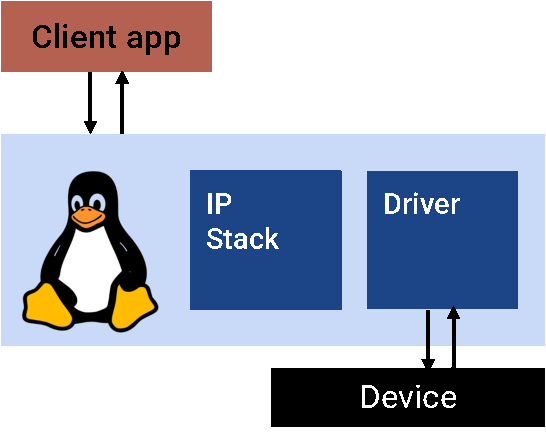
\includegraphics[width=6cm]{sockets.pdf}
	\caption{Network packet processing in a monolithic kernel.}
	\label{f:sockets}
\end{figure}

A monolithic operating system houses both drivers and protocol stacks in kernel as shown in
\autoref{f:sockets}. These components are typically written as libraries for the kernel to 
process a packet. In order for
a user application to utilise the network, the application must open a socket through a system
call. This system call creates an endpoint for communication and returns a file descriptor that refers
to that endpoint \cite{Linux:socket}. The file descriptor can then be used to read (receive a packet)
or write (transmit a packet) to the socket using the protocols specified when opening the socket.

To receive a packet on the network, the OS must first enqueue the addresses of buffers in memory to 
the device's control registers. The device can then write newly received data directly to these buffers. 
Once a packet has been written, the device will issue an interrupt to the OS to notify the OS. The 
kernel then processes this packet as defined by the IP protocol used in the packet. This typically 
includes reading the packet header, which contains critical information such as where the packet has
come from, where it is headed, as well as the communication protocol used. This information advises the
kernel about what to do with the packet. If the packet is addressed to a user-level application bound to
a socket, eventually the header of the packet will be stripped before the data is copied to a user space 
buffer queue attached to the socket. This buffer can now be accessed using a read (\emph{recv()}) system 
call. Note that much like a file read system call, this system call will block until there is data
available to be read.

To transmit, a user application can write a packet using a write (\emph{send()}) system call. 
The data will first be copied into an in kernel buffer. The kernel will process 
the packet and an appropriate header will be added to the head of the packet as per the protocol used 
with the socket. Eventually, this kernel buffer address will be enqueued to the device control
registers which signals to the device that a packet is ready for transmit, after which, the system call
returns. Once the device has transmitted the packet, it will issue an interrupt to notify the kernel
that the buffer is no longer in use and can be re-used.

Operating systems commonly use interrupt hold off on the device as an attempt to batch hardware
events, such as receiving or transmitting a packet, into a single interrupt. This means that the kernel
will be able to more efficiently process multiple packets at a time. At high throughputs on the receive
path, the kernel will even disable receive interrupts and switch to polling mode instead. This removes
the interrupt handling overhead but requires the driver to continuously check for hardware events.
Furthermore, in recent years, hardware has become more complex, and network devices are capable of 
commandeering some of the packet processing. This includes, for example, computing the packet
checksum or packet coalescing. Many of such hardware extensions have been capitalised on by monolithic
kernels to reduce the software overhead of packet processing.

%%%%%%%%%%%%%%%%%%%%%%%%%%%%%%%%%%%%%%%%%%%%%%%%%%%%%%%%%%%%%%%%%%%%%%%%%%%%%%%%%%%%%%%%%%%%%%%%%%%%%%%%%%%%%%%%%%%%%

However, the typical method of networking in a monolithic kernel is both insecure, due to the amount 
of untrusted code running at privilege level, and performs poorly, due to data copying operations and 
the increasing cost of system calls, particularly
those used for sending and receiving a packet \cite{Ren_RCVSY_19}.

\section{seL4}
\begin{figure}[h]
    \centering
    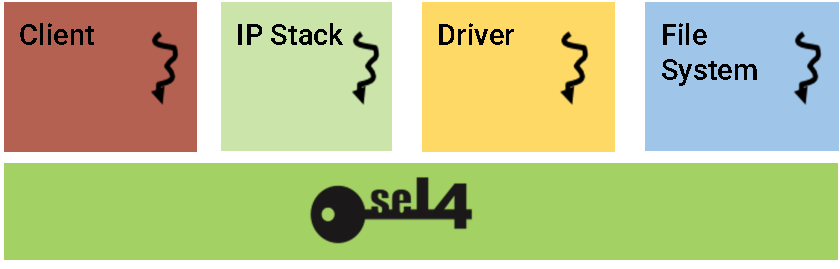
\includegraphics[width=8cm]{seL4.pdf}
    \caption{seL4 architecture}
    \label{f:sel4}
\end{figure}

seL4 is a highly performant, highly secure microkernel. It has been formally verified to be
functionally correct down to the binary, along with upholding the security properties confidentiality, 
integrity and availability \cite{Klein_AEMSKH_14}. However, as a microkernel, it provides only the minimum
to securely abstract the hardware and nothing more \cite{Heiser_PCVL_22}. As such, 
it presents a very low level API, and it does not provide resource management, file systems, network stacks
or device drivers and instead prescribes these services to run as user level programs. 
The kernel makes no distinction between such services and applications, which results in the horizontal
architecture shown in \autoref{f:sel4}. 

seL4 is also a capability based system. A capability is a communicable, unforgeable token that 
references a kernel object with an associated set of access rights. This provides fine grained access control
and means user-level components must have a capability in order to access an object and means that seL4
guarantees components only have access to objects, including data, that developers permit them to.
Additionally, seL4 guarantees ensure full isolation of user-level components, meaning that
failure of any component is completely contained and will not bring the rest of the system down. 
Finally, seL4 is the worlds fastest microkernel and performs within 25\%
of the limits imposed by hardware \cite{Mi_LYWC_19}. 

However, the microkernel design can potentially degrade performance as it requires
significantly more context switches than its monolithic counterpart. This is because OS services,
such as device drivers, typically run as an isolated components, and client
applications wishing to use such services must communicate using synchronous/asynchronous
IPC and shared memory. Furthermore, interrupt processing is forwarded to the user level handler
through asynchronous system calls and user level applications are also responsible for initiating
any cache management operations through system calls when required
for memory consistency. These system calls, which aren't typically required in a monolithic
system, can quickly add up. 

% Core Platform
\section{The seL4 microkit}
The seL4 microkit, formerly known as the seL4 Core Platform,
is an operating system framework on seL4 with minimal abstractions over seL4 low level
objects \cite{Heiser_PCVL_22}. It aims to ease the development process of applications on seL4 by abstracting over
architecture specific details as well as seL4's low level API. Microkit trades generality for simplicity and 
restricts systems to a predominantly static architecture. This means components are fixed at build time. 
The abstractions are:
\begin{enumerate}
    \item \textbf{Protection Domain (PD)}: a process abstraction that enforces an event driven programming model.
    \item \textbf{Communication Channel (CC)}: the ability for two PDs to communicate via notifications or PPCs.
    \item \textbf{Memory Region (MR)}: a range of physical memory that may be mapped into 1 or more PDs address spaces. 
    \item \textbf{Notification}: a semaphore-like synchronisation primitive. 
    \item \textbf{Protected Procedure Call (PPC)}: synchronous RPC between PDs. 
\end{enumerate}

Microkit promotes the correct use of seL4 by employing an event driven driven programming model for PDs. Events are triggered by
either notifications or PPCs sent along a CC. Microkit also restricts the use of seL4's IPC primitives to remote procedure calls,
which is only possible if the callee has strictly higher priority than the caller. This prevents PDs from either directly or 
indirectly calling themselves. Finally, while microkit predominantly only supports static systems, there is 
some supported dynamism which enables the re-initialising of PDs and dynamically loading code into PDs \cite{Heiser_PCVL_22}.

\chapter{Related Work}\label{ch:related_work}

The wider community is well aware of the problem space created by untrusted/unreliable
code running inside the kernel and there have been a variety of attempts to deprivilege
components and/or improve the performance in networking-focused systems.
In \autoref{s:async} we explore new asynchronous APIs to minimise the system call overhead. In 
\autoref{s:userspace_dd} we examine user level I/O frameworks that bypass the OS altogether
to deprivilege device drivers and remove the system call overhead. Finally, in \autoref{s:isolation_dd}
we consider isolation techniques that take advantage of hardware virtualisation support to remove
drivers from the TCB.

\section{Asynchronous I/O Frameworks}\label{s:async}
In order to combat the performance overheads of typical network packet processing, a number of new APIs
have been developed with an asynchronous programming model.

\subsection{Netmap}\label{netmap}
Netmap aims to decrease packet processing costs on monolithic kernels through an asynchronous, zero copy 
API \cite{Rizzo_12}. Specifically, netmap removes the cost of dynamically allocating buffers per packet by 
preallocating fixed size packet buffers when the network device is first opened. These buffers are
shared between kernel and user space to remove the cost of data copying operations. Finally,
netmap removes the cost of blocking system call operations by providing an asynchronous API to user level applications. 
Applications open a special device file \lstinline{/dev/netmap} using \emph{ioctl()} and a flag to indicate registration.
This function will return the size of the memory region containing shared data structures for buffer management.  
On the receive path, another \emph{ioctl()} system call with the receive flag will return the number of packets available 
for reading. These packets can then be found in buffers ready to be dequeued from a shared receive queue. 
On the transmit path, applications write packets intended for transmit into shared buffers and insert into the shared transmit 
queue. Another \emph{ioctl()} system call is used with the transmit flag to notify the OS about the new 
packets to send. Importantly, the \emph{ioctl()} call with either the receive or transmit flag is non blocking.
This asynchronous interface is able to significantly reduce the system call overhead by providing a simple mechanism
to batch packet processing. With this, the netmap API achieves significantly higher transmit throughput than the
socket API.

\subsection{io\_uring}\label{io_uring}
\lstinline{io_uring} is another asynchronous API for I/O frameworks on Linux \cite{io_uring}. 
As opposed to netmap, \lstinline{io_uring} provides a more generalised interface for different 
classes of I/O processing and not just network-based applications. \autoref{f:fio_uring} shows the 2 shared
ring buffers between kernel and user space: one for submitting a request, another for results of completed requests. 
These ring buffers are set up using \emph{io\_uring\_setup()} and then mapped into user space with \emph{mmap()}. 
To issue a read or write request, applications must provide a user level buffer, set appropriate flags in the submission
queue entry and add this entry to the tail of the requests ring buffer. User applications inform
the kernel of updates to the requests ring buffer using a new system call \emph{io\_uring\_enter()}. This system call is blocking, 
and returns once the kernel has processed the new requests and the results are available in the completed queue. 
To provide an asynchronous interface, there is an optional polling mode, whereby the kernel will continue to poll for updates
in the requests queue. Polling mode removes the need for system calls, which can significantly improve throughput.

\begin{figure}[h]
	\centering
	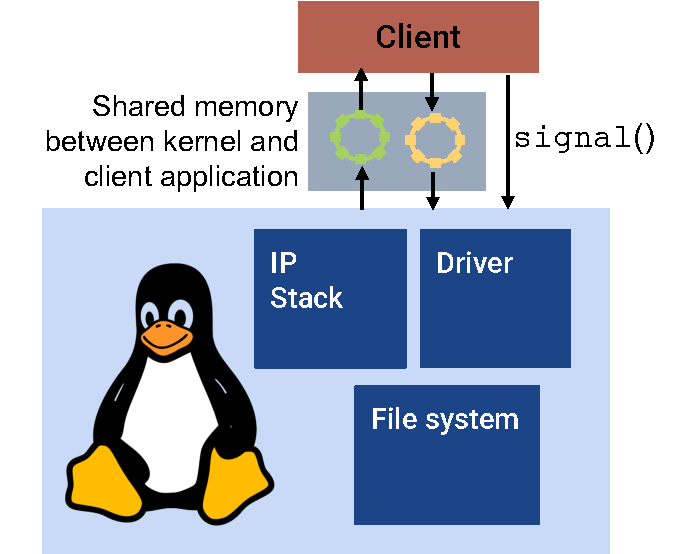
\includegraphics[width=7cm]{io_uring.pdf}
	\caption{System design with io\_uring.}
	\label{f:fio_uring}
  \end{figure}

\subsection{Takeaways}
Both netmap \cite{Rizzo_12} and \lstinline{io_uring} \cite{io_uring} reduce performance overheads of I/O on monolithic kernels
by providing an asynchronous interface to enable batching, or the complete removal of system calls. However, both APIs 
rely on in-kernel device drivers and do not explore the security vulnerabilities of such a design. 
Furthermore, netmap requires exclusive device access and thus the usual in-kernel device sharing mechanisms do not work. 
Instead, if the NIC is to be shared, the pool of data buffers will be mapped into every user process that shares the NIC. 
The result is that a process has access to data belonging to other processes. Also, the polling mode of
\lstinline{io_uring} would monopolise the CPU even when there is no work to be done, consequently driving up
power consumption of the system and it is unclear what policy is applied to this mode when there are multiple client
applications using it, or if there is other work to be done by the kernel.

\section{User space device drivers}\label{s:userspace_dd}
Running device drivers as user level programs is the simplest way to deprivilege the software and provide
strong fault isolation. However, this can lead to a significant increase in the number of system calls
required and this cost can degrade performance significantly. In order to overcome this, kernel bypass
frameworks have been developed to support user level IO asynchronously.

\subsection{DPDK}\label{dpdk}
DPDK (Data Plane Development Kit) provides data management libraries along with a set of network drivers to offload
network packet processing to user space and bypass the OS in a Linux environment \cite{DPDK:wp_20}. \autoref{f:dpdk}
shows the system design differences between using an in kernel network driver vs a DPDK library.

\begin{figure}[h]
  \centering
  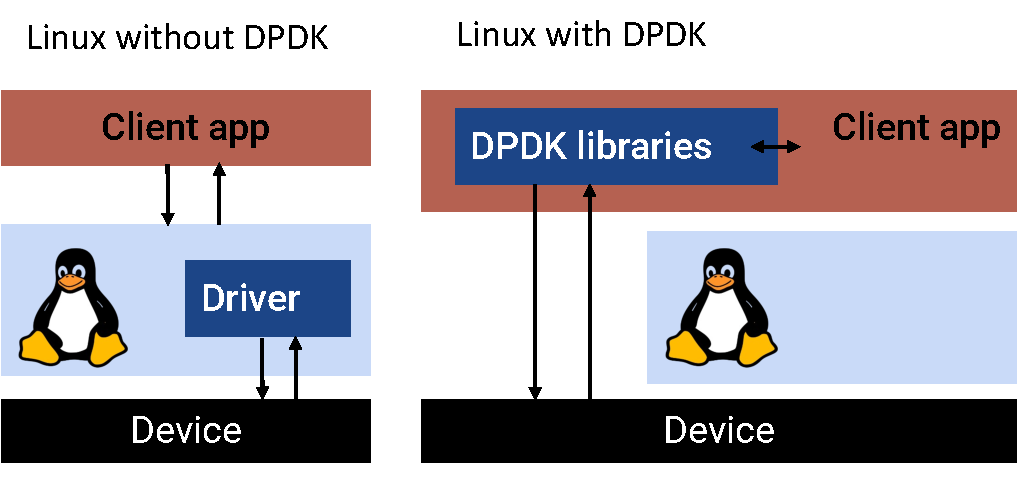
\includegraphics[width=10cm]{dpdk.pdf}
  \caption{System design without and with DPDK.}
  \label{f:dpdk}
\end{figure}

Specifically, it provides \cite{DPDK:wp_20}:
\begin{itemize}
	\item Lock free, bounded, multi producer, multi consumer (MPMC) ring buffer queues for efficient data management.
	\item Buffer management to preallocate fixed sized buffers.
	\item A library of polling mode drivers.
\end{itemize}

DPDK enables faster packet processing than a typical in-kernel driver as it removes the cost of context switching
between kernel and user space. Instead of receiving an interrupt, drivers must poll for hardware events. 
This means the driver needs to continuously read the device's event register. This has the consequence of driving
the CPU utilisation of the system up as the system cannot be idle while waiting for an event. 
In addition, the framework itself is zero copy, so DPDK can further reduce packet processing costs as it no longer needs to copy 
packet data into and out of user space. Finally, the framework uses huge pages for large memory pools, 
which decreases the amount of look-ups and other page management costs while ensuring relevant pages stay pinned in memory and
aren't migrated in the background due to Linux's page migration policy.

\subsubsection{BBQ}
BBQ is a block-based bounded queue design that aims to increase performance of ring buffer queues in frameworks such
as DPDK \cite{Wang_BFOOLCHC_22}. DPDK uses multi producer, multi consumer queues, which are designed with the
intention to split the workload across several processors. However, these queues have cache interference when
performing consecutive operations and this degrades performance. This stems from the MPMC queue design as it needs to keep track of
two heads and two tails to keep track of where a producer can produce to without interference from another producer (and
likewise for consumers). Pseudo code for interacting with MPMC queues is shown \autoref{l:prod} and \autoref{l:cons} 
\cite{Wang_BFOOLCHC_22}.

\noindent\begin{minipage}{.45\textwidth}
\fontsmall
\begin{lstlisting}[numbers=left, tabsize=2, language=C, caption={Producer pseudo code},frame=tb, label={l:prod}, captionpos=b]
  enqueue(data) {
  again:
  	ph = load(prod.head)
  	pn = ph + 1
  	if (pn > load(cons.tail) + SIZE)
  		return FULL
  	if (!cas(prod.head, ph, pn))
  		/* Another producer is 
  		   using this slot */
  		goto again
  	entry[pn] = data
  	/* Wait until earlier slots have
  	   successfully committed */
  	while(load(prod.tail) != ph)
  	store(prod.tail, pn)
  	return OK
  }
\end{lstlisting} 
\end{minipage}\hfill
\begin{minipage}{.45\textwidth}
\fontsmall
\begin{lstlisting}[numbers=left, tabsize=2, language=C, caption={Consumer pseudo code},frame=tb, label={l:cons}, captionpos=b]
  dequeue() {
  again:
  	ch = load(cons.head)
  	cn = ch + 1
  	if (cn > load(prod.tail))
  		return EMPTY
  	if (!cas(cons.head, ch, cn))
  		/* Another consumer is 
  		   consuming this slot */
  		goto again
  	data = entry[cn]
  	/* Wait until earlier slots have 
       successfully committed */
  	while(load(cons.tail) != ch)
  	store(cons.tail, cn)
  	return data
  }
\end{lstlisting}
\end{minipage}

The performance degradation comes from two possible places:
\begin{enumerate}
\item Cache misses occur in a multiprocessing environment every time a producer reads the
consumer's tail (on line 5 in \autoref{l:prod}), even though the tail might be far behind and not
of concern. This is because the cache belonging to the core running the producer will not have the
required data and it must be fetched from the owner (either from main memory or the local cache of
a core running a consumer). Likewise, the consumer will also always miss on the 
producer's tail (on line 5 in \autoref{l:cons}) although it may be far ahead.
\item When multiple threads try to read the same entry, they must continuously try again as shown at lines 7 - 10 in 
\autoref{l:prod} and \autoref{l:cons}
\end{enumerate}

BBQ proposes a block-based approach instead, where the queues are divided into blocks and the producers only
start using a block once it has been fully consumed. This avoids the cache miss on 
reading the consumer's tail. Each block contains 4 variables to keep track of the actions: allocated,
committed, reserved and consumed. Producers produce between allocated and committed, but these variables 
aren’t updated until the block is fully consumed (this is to prevent cache misses by the consumer).
Compared with DPDK, BBQ isn't as affected by CPU over-subscription. This is because in the MPMC
DPDK queues, the producers can form a waiting chain, where the last thread to allocate an entry can only 
commit that entry once the previous thread has committed its entry. While this waiting chain would have 
minimal impact if the threads are scheduled in the optimal order to each make progress, this is often not 
the case. As producers in BBQ commit independently using an atomic Fetch-and-Add 
instruction, this scenario does not occur.\\
Overall, the BBQ approach attempts to solve performance issues of MPMC queues in a multiprocessing environment,
which stem from the concurrency involved in such queues. 

\subsubsection{CleanQ}
CleanQ takes the opposite approach of BBQ and instead outlines the need for a simple and \emph{reliable} ring buffer
design that does not impede performance in frameworks such as DPDK \cite{Haecki_HACSR_19}. CleanQ removes
the inherent complexity of MPMC queues and instead returns to single producer, single consumer (SPSC)
queues. These queues are significantly simpler, and as a result, Haecki et. al. are able to infer
correct guarantees from the design. CleanQ uses the concept of `ownership' to base their formal invariants. 
Consider `entities' to be either a producer or a consumer acting on the queues and `objects' to be items passed around
by these queues, then the invariants guaranteed by the CleanQ design are:
\begin{enumerate}
\item An object has at most one owner,
\item If an entity owns an object, it has exclusive use of it,
\item An entity knows whether it owns an object or not,
\item Ownership can be transferred.
\end{enumerate}
These guarantees eliminate many subtle bugs in lock-free queue design.
Furthermore, the CleanQ design achieves higher throughput than DPDK MPMC queues in a networking
context, which ultimately highlights that a simple design does not negatively impact performance.

\subsubsection{Takeaways}
DPDK completely bypasses the OS to offload packet processing to user space. The zero copy design in user space
achieves higher throughput than typical in-kernel packet processing\cite{DPDK:wp_20}. However, all drivers 
are polling mode only. This design decision stems from the high cost of interrupt handling on Linux, but it enables
the application to monopolise the CPU as the driver must continuously poll for events. While the polling has little
impact in high throughput networking scenarios where there is consistently work to be done, at lower throughput,
the CPU utilisation will not decrease with the workload and the system will maintain high power consumption without
making progress. Moreover, implementing a device driver as a library inside an application limits the device to a
single client. Ultimately, the short-comings of monolithic kernels, namely, the high cost of interrupt processing
and context switching, have influenced the design and reduced the flexibility. DPDK also relies on cache-coherent
architectures to achieve performance, as the minimal support available for cache management operations from userspace
introduces costly system calls. Finally, MPMC queues used in the DPDK data plane are inherently complex due to the 
concurrency involved and have the potential to degrade performance \cite{Wang_BFOOLCHC_22}. The simpler and
cleaner design of ring buffer queues as shown in CleanQ, can not only achieve higher throughput, but are also
verifiable \cite{Haecki_HACSR_19}.

\subsection{Ixy}
Ixy is a user-space packet framework on Linux that aims to educate developers on driver development 
\cite{Emmerich_PBHZC_19}. It utilises the \emph{uio} and \emph{vfio} interfaces to access the device from
user space. Using these APIs, Ixy develops a user space polling mode device driver for the ixgbe 10Gbps
NIC with low packet forwarding costs. Significantly, the ixy device driver reduces the \emph{ixgbe}
in-kernel driver from over 10K LOC to just over 1K LOC.

\subsubsection{Linux uio}
\emph{uio} (User space I/O) exposes interfaces for user level device drivers by memory mapping files in the \emph{sysfs}
pseudo file system on Linux \cite{UIO}. Interrupts are handled by reading this file once mapped. For example,
a \emph{read()} system call will block until an interrupt is triggered. The integer value read from this file represents
the total interrupt count. \emph{uio} exposes the device registers via \emph{mmap()} when using a particular offset calculated
based on the number of devices using \emph{uio}. However, \emph{uio} hides the issue that DMA 
addresses must stay in resident memory and that Linux page migration does not guarantee that physical addresses
won't change behind the scenes. To overcome this issue, \emph{uio} users can use
huge pages as these won't be migrated by the Kernel.

\subsubsection{Linux vfio}
\emph{vfio} (Virtual Function I/O) extends \emph{uio} and adds support for IOMMU use \cite{VFIO}. The IOMMU is a memory
management unit mapping device-visible virtual addresses to physical addresses, and lies on the system bus between I/O devices
and main memory. When used, the main advantage of the IOMMU is protecting memory from malicious/faulty devices attempting
errant memory accesses. \emph{vfio} introduces additional
files in the \emph{sysfs} file system to expose the IOMMU to user space and provides data structures and library functions
that can be used to map/unmap memory in the IOMMU for safe DMA through \emph{ioctl()} system calls on Linux.

\subsubsection{Takeaways}
Although the ixy user level device driver is not as performant as its counterpart on the DPDK framework, it reduces a
large and complex device driver to a much smaller driver without significant performance degradation. The lower
performance of ixy when compared to DPDK can in part be attributed to DPDK's use of SIMD instructions to handle
batches of packets at a time \cite{Emmerich_PBHZC_19}. SIMD units are hardware components that perform the same
operation on multiple data operands concurrently. In packet processing, this parallelism can boost performance
on checksum calculations. However, much like DPDK, ixy is reliant on cache coherent architectures and also does
not support device sharing.

\subsection{Snap}\label{snap}
Snap proposes a modular architecture, comparable to a microkernel design, by utilising asynchronous communication
mechanisms and minimal state sharing \cite{Marty_dKAABCDDEGKKKMMORRSTVWV_19}. The design intentionally leans away 
from typical socket programming for networking systems and instead opts for an event driven model. They present
a user space network driver that uses asynchronous communication and ring buffers in shared memory for data transfer.
Interrupts are delivered to an event file, which can be polled from user
level. Alongside this, Snap takes a unique approach to scheduling. Rather than
designing a generic scheduling policy that aims to be applicable across a large set of scenarios, they instead propose 3
different designs that could be swapped as required:
\begin{enumerate} 
\item Tasks are pinned to cores to take advantage of cache efficiency.
\item Tasks are spread dynamically. Threads are scheduled when interrupts are delivered to process the event on
the next available core.
\item Tasks are spread dynamically as above but onto as few cores as possible. This aims to take advantage
of cache efficiency when possible, but as work queues up, the allocation needs to be queried. 
\end{enumerate}

\subsubsection{Takeaways}
The Snap design deprivileges untrusted drivers by running them in user space and the design, although running on top
of a monolithic kernel, uses event driven programming. This design is shown to scale well to multiple clients and the
swappable scheduling policy removes complexity from the trusted computing base while demonstrating efficiency.

\subsection{Microdrivers}
Instead of running the entire driver at user level, Microdrivers split the device driver into two separate
components; one of which runs at kernel level and the other at user level in order to achieve the performance 
of in kernel drivers combined with the fault isolation of user level drivers 
\cite{Ganapathy_RBSJ_08}. \autoref{f:microdrivers} shows the architecture of microdrivers. 
The kernel mode component contains performance critical and frequently used 
functionality. For a network driver, this includes interrupt handling and sending and 
receiving packets. The rest of the code, predominantly initialisation and error handling, goes into user level 
where the performance degradation of context switching between kernel and user level does not have noticeable
impact. In order to speed up the user mode component, microdrivers duplicate functions
in both components and use shared memory for frequently accessed data structures.

\begin{figure}[h]
  \centering
  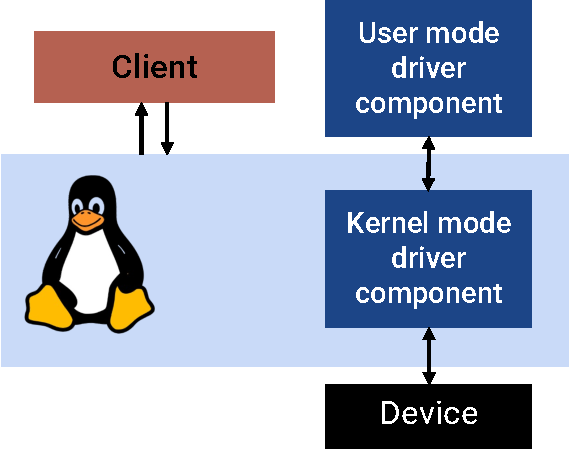
\includegraphics[width=8cm]{microdrivers.pdf}
  \caption{Microdrivers architecture}
  \label{f:microdrivers}
\end{figure}

\subsubsection{Takeaways}
Although 70\% of driver code consists of non-performance-critical functions and can be relegated to user space
\cite{Ganapathy_RBSJ_08}, this does not provide good fault isolation. The remaining 30\% of driver code is 
just as untrustworthy, and faults have higher impact as this code is on the critical path. Furthermore, by sharing
data structures between kernel and user space, some of which could contain sensitive kernel data, higher trust 
needs to be placed on the user mode component, thus diminishing any safety guarantees obtained by running the 
code at user level. Finally, the research was not able to produce reliable performance results which undermines
any performance gains of running part of the driver at kernel level. Thus, splitting a driver into a user level
component and a kernel level component is not viable and could achieve the worst of both designs: poor performance
and poor fault isolation.

%%%%%%%%%%%%%%%%%%%%%%%%%%%%%%%%%%%%%%%%%%%%%%%%%%%%%%%%%%%%%%%%%%%%%%%%%%%%%%%%%%%%%%%%%%%%%%%%%%%%%%%%%%%%%%%%%%%%%

\section{Isolating Kernel Components inside the OS}\label{s:isolation_dd}
Another method to deprivilege untrusted code inside the OS is to use isolation techniques. These approaches
rely on hardware virtualisation extensions in order to re-use legacy code and avoid the redesign and redevelopment
of OS components like drivers while also supporting device sharing.

\subsection{Nooks}
A Nook provides an isolated environment for driver execution inside a monolithic OS \cite{Swift_MLE_02}. The
driver still runs inside the kernel address space, but within a different protection domain. This can be achieved
using virtual memory protection and lowering the privilege level to remove access to privileged instructions. 
For shared resources, the OS can call into isolated device drivers with a wrapper function in order to track 
resource usage, verify data passed in/out, flush the TLB and perform a software trap. Similarly, a driver
accessing a shared data structure is trapped so the OS can update the data on the drivers behalf.

\subsubsection{Takeaways}
Unfortunately there is a lack of detail into the Nooks architecture and the work doesn't account for potential 
performance degradation due to some of the design decisions. Firstly, in order for the OS to update data on the drivers
behalf, it would need to first verify this data. How this data is verified and to what extent could cost cycles on a 
critical path. Furthermore, interrupts are forwarded to the isolated driver. Nooks measured 
interrupt handling on a isolated driver to cost double the cycles of an in kernel driver, yet 
there is no accounting for this in the performance. This cost is significant and would limit drivers to polling
mode only.

\subsection{{LXDs}}
LXDs (Lightweight Execution Domains) enable isolation in a monolithic OS using hardware-assisted virtualisation
(VT-x) \cite{Narayanan_BJSBQ_19}. The design utilises a small microkernel that runs inside the monolithic OS to
provide both synchronous and asynchronous communication channels between kernel processes and isolated components.
\autoref{f:lxds} outlines the architecture of this solution. Instead of a typical function call to transmit data 
that would call into an in-kernel driver library, it instead sends a message via the LXDs microkernel to the
isolated driver. The isolated driver has direct access to the NIC and can then perform the transmit. 

\begin{figure}[h]
  \centering
  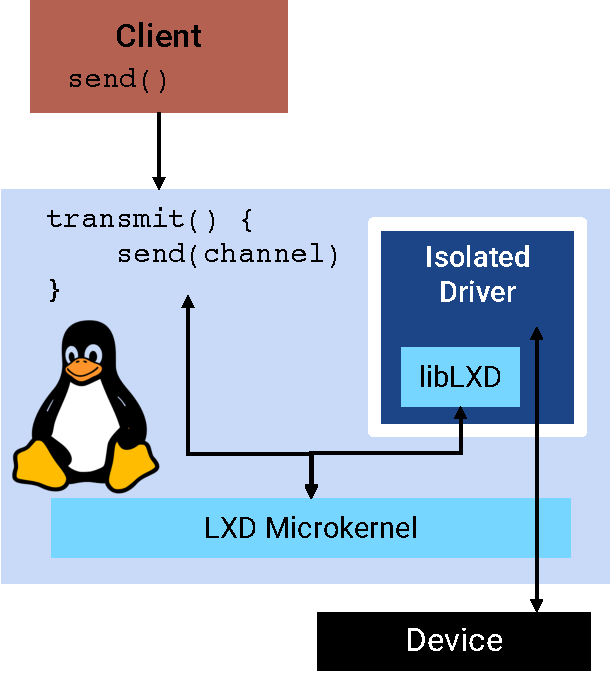
\includegraphics[width=7cm]{LXDs.pdf}
  \caption{System design of LXDs with an isolated NIC driver}
  \label{f:lxds}
\end{figure}

In order to achieve this design, they prescribe methods to decompose kernel code to help analyse the 
interaction patterns between the kernel and its drivers. They propose a new IDL (Interface Definition 
Language) to auto generate glue code based on these patterns. This glue code creates copies
of shared data structures to ensure such structures aren't shared between domains, and translates function calls into 
an isolated domain into remote procedure calls \cite{Narayanan_BJSBQ_19}.\\ 
To better isolate device drivers, the design pins a driver to a particular core and enables communication via cross-core
message passing. Synchronous message passing via the LXDs microkernel is used initially for establishing regions of
shared memory that are then set up for asynchronous communication in the form of ring buffer queues. Cross-core communication
then just relies on cache coherence, which has a lower cost (around 380 cycles) than using hardware mechanisms for
address space isolation (around 850 cycles)\\
Instead of blocking waiting for another core running an isolated driver to complete its work, the design proposes to instead
spawn a light weight thread when communicating asynchronously that can wait for the response. The original thread
can then keep executing. When this is not possible, for example, when the next instruction relies on the result of the call,
continuations can be used as well. 

\subsubsection{Takeaways}
Although the design was able to achieve throughput within 80\% of a non-isolated NIC driver,
the design has several limitations. Firstly, the design relies on utilising multiple cores to achieve comparable
performance. This is not always practical, and has the potential to waste resources. Although the paper does not display
CPU utilisation figures for their benchmarks, by pinning a polling driver to a particular core, even at low loads 
this core will be executing at 100\%. Additionally, the architecture involves adding a microkernel type
component to the trusted computing base inside the OS. Although it may be small, there is no comment on the
complexity of this new addition and this extra layer must be trusted in order to remove the driver from the TCB.
This design also introduces more concurrency into the kernel by spawning threads to wait for cross-core communication.
Finally, the research is limited to device drivers on multicore hardware and does not include other
layers and components in the networking processing plane such as the IP stack. The Linux kernel IP stack is significantly
more complex and difficult to isolate in such a manner.

\subsection{Isolation using VMFUNC}
Another method of isolating drivers and other kernel extensions is to use recent hardware mechanisms such as VMFUNC and
extended page table switching. This design involves executing the OS on top of a minimal hypervisor to make use of 
these hardware mechanisms \cite{Narayanan_HTJB_20}. VMFUNC is an Intel primitive that changes the extended page table
underneath a virtual machine without exiting into the hypervisor. As the VMFUNC instruction is significantly faster than
switching privilege levels, this research proposes using this instruction in a trampoline mechanism to quickly context switch
into an isolated component. \autoref{f:vmfunc} demonstrates the overall architecture. Similarly to the LXDs architecture,
the in kernel driver is replaced by stub code that crosses the isolation boundary using vmfunc trampoline code before
performing the transmit on the device.

\begin{figure}[h]
  \centering
  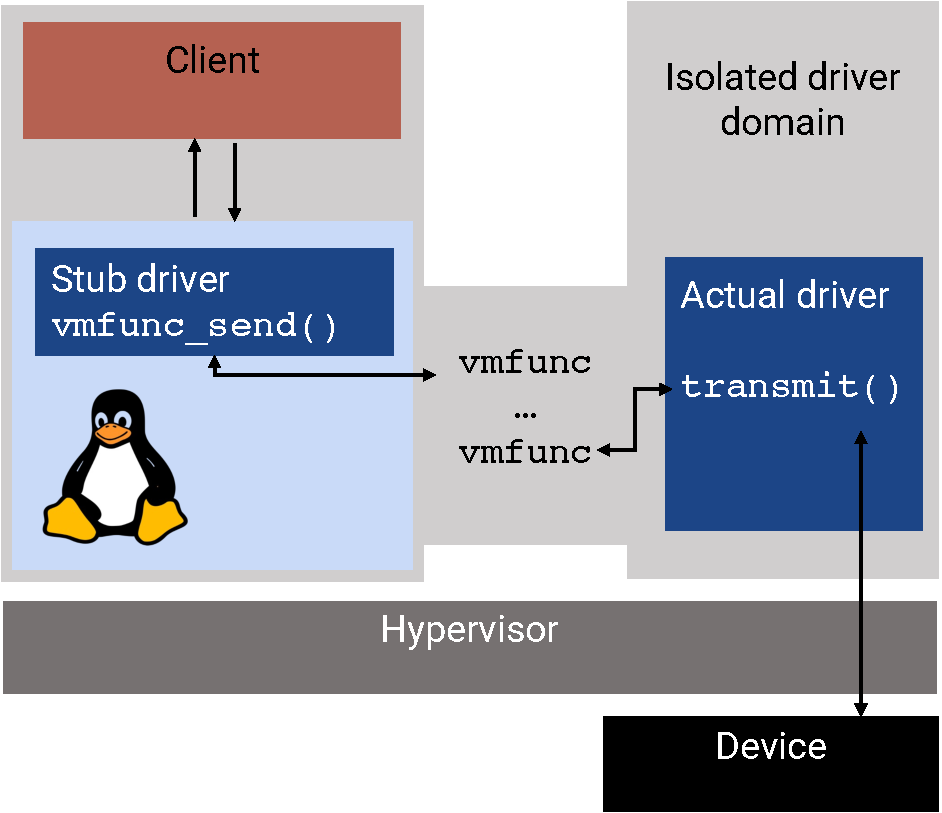
\includegraphics[width=10cm]{vmfunc.pdf}
  \caption{System design using vmfunc trampoline to isolate NIC driver}
  \label{f:vmfunc}
\end{figure} 

However, this architecture is not necessarily secure and extra measures must be taken. These are:
\begin{enumerate}
	\item Ensure virtual address spaces of isolated domains, kernel and user processes do not overlap. This is to prevent a 
	malicious component from executing VMFUNC on its own accord and having the ability to access to data it should not. 
	The same applies to physical addresses.
	\item ensure isolated domains have read-only access to their page table. This is to ensure an isolated component cannot
	change its address space layout and thus violate the above.
	\item Sensitive data is protected by either mediating it through the hypervisor (such as control registers) or saved and 
	restored across domain switches (general, segment and extended state registers). This happens in the trampoline code.
\end{enumerate}

\subsubsection{Takeaways}
Isolating a network driver using the above design achieved throughput within 1\% to 11\% of the native polling driver on a
10Gbps NIC. Although the isolation technique used seems to add minimal overhead, some overhead is hidden in the interrupt
delivery for non-polling drivers. The design proposes mapping the interrupt descriptor table is into both the kernel
and the isolated domains to prevent the need to trap into the hypervisor on interrupt. The interrupt is
then first handled by the kernel domain before interrupting the isolated driver where applicable. 
However, this allows an untrusted component access to the interrupt descriptor table and the ability to disable interrupts 
and never return control to the OS. To overcome this, they propose using a preemption timer in the hypervisor to ensure the 
kernel domain is making progress. Overall, the cost of delivering an interrupt to an isolated 
domain is over 1000 cycles, and the cost and trade-offs of using a preemption timer
in the hypervisor is not measured. Furthermore, to ensure an untrusted isolated component did not alter the interrupt
descriptor table without disabling all interrupts (eg. it could disable interrupts of some other device), the OS would
need to check the interrupt descriptor table on every return. This cost is not measured. Overall, mapping the interrupt
descriptor table into untrusted domains is inherently insecure and should be avoided. 

% RedLeaf? 
\section{Summary}
Typical network packet processing is both insecure and non-performant. This is because complex, bug prone software systems
run in the trusted computing base, and the complexity of such systems has led to reduced performance. The solutions outlined above
aim to rectify this, but are largely limited by the monolithic kernel design itself. 
Asynchronous IO frameworks improve performance without addressing the security vulnerabilities. User level drivers
achieve high throughput at the cost of high utilisation and are limited to single client applications. Although techniques to
isolate drivers inside the OS promote device sharing, these techniques are not extensible to other kernel subsystems, they
do not completely protect the OS and can also degrade performance. However, there are still some significant
learnings we can take away from the above work. Firstly, Rizzo (2012), Axboe (2019), Linux Foundation (2020) and Marty et al. (2019)
demonstrate significant performance gains through the use of an asynchronous API. Emmerich et al. (2019) showed that a complex
device driver for a high throughput NIC could be simplified 10 fold and still achieve performance. Haecki et al. (2019)
demonstrated that simple SPSC queues can outperform complex MPMC queues, and Marty et al. (2019) demonstrated that a
modularised approach with flexible policy achieves competitive throughput in a real world application of data centres.

\chapter{The seL4 Device Driver Framework}\label{ch:sddf}
Unfortunately, many approaches to solving the issues with I/O are limited 
by the monolithic kernel design itself. This presents a strong argument to
redesign a performant yet secure I/O framework on a different architecture completely: the microkernel.
However, the microkernel design has the potential to degrade performance as it requires
significantly more context switches than its monolithic counterpart.
In order to overcome potential performance degradation in I/O systems due to this, we require a simple
framework that minimises system calls when possible for designing performant I/O systems on a microkernel architecture.
This introduces the seL4 Device Driver Framework as an excellent starting point for this project.\\

\begin{figure}[h]
    \centering
    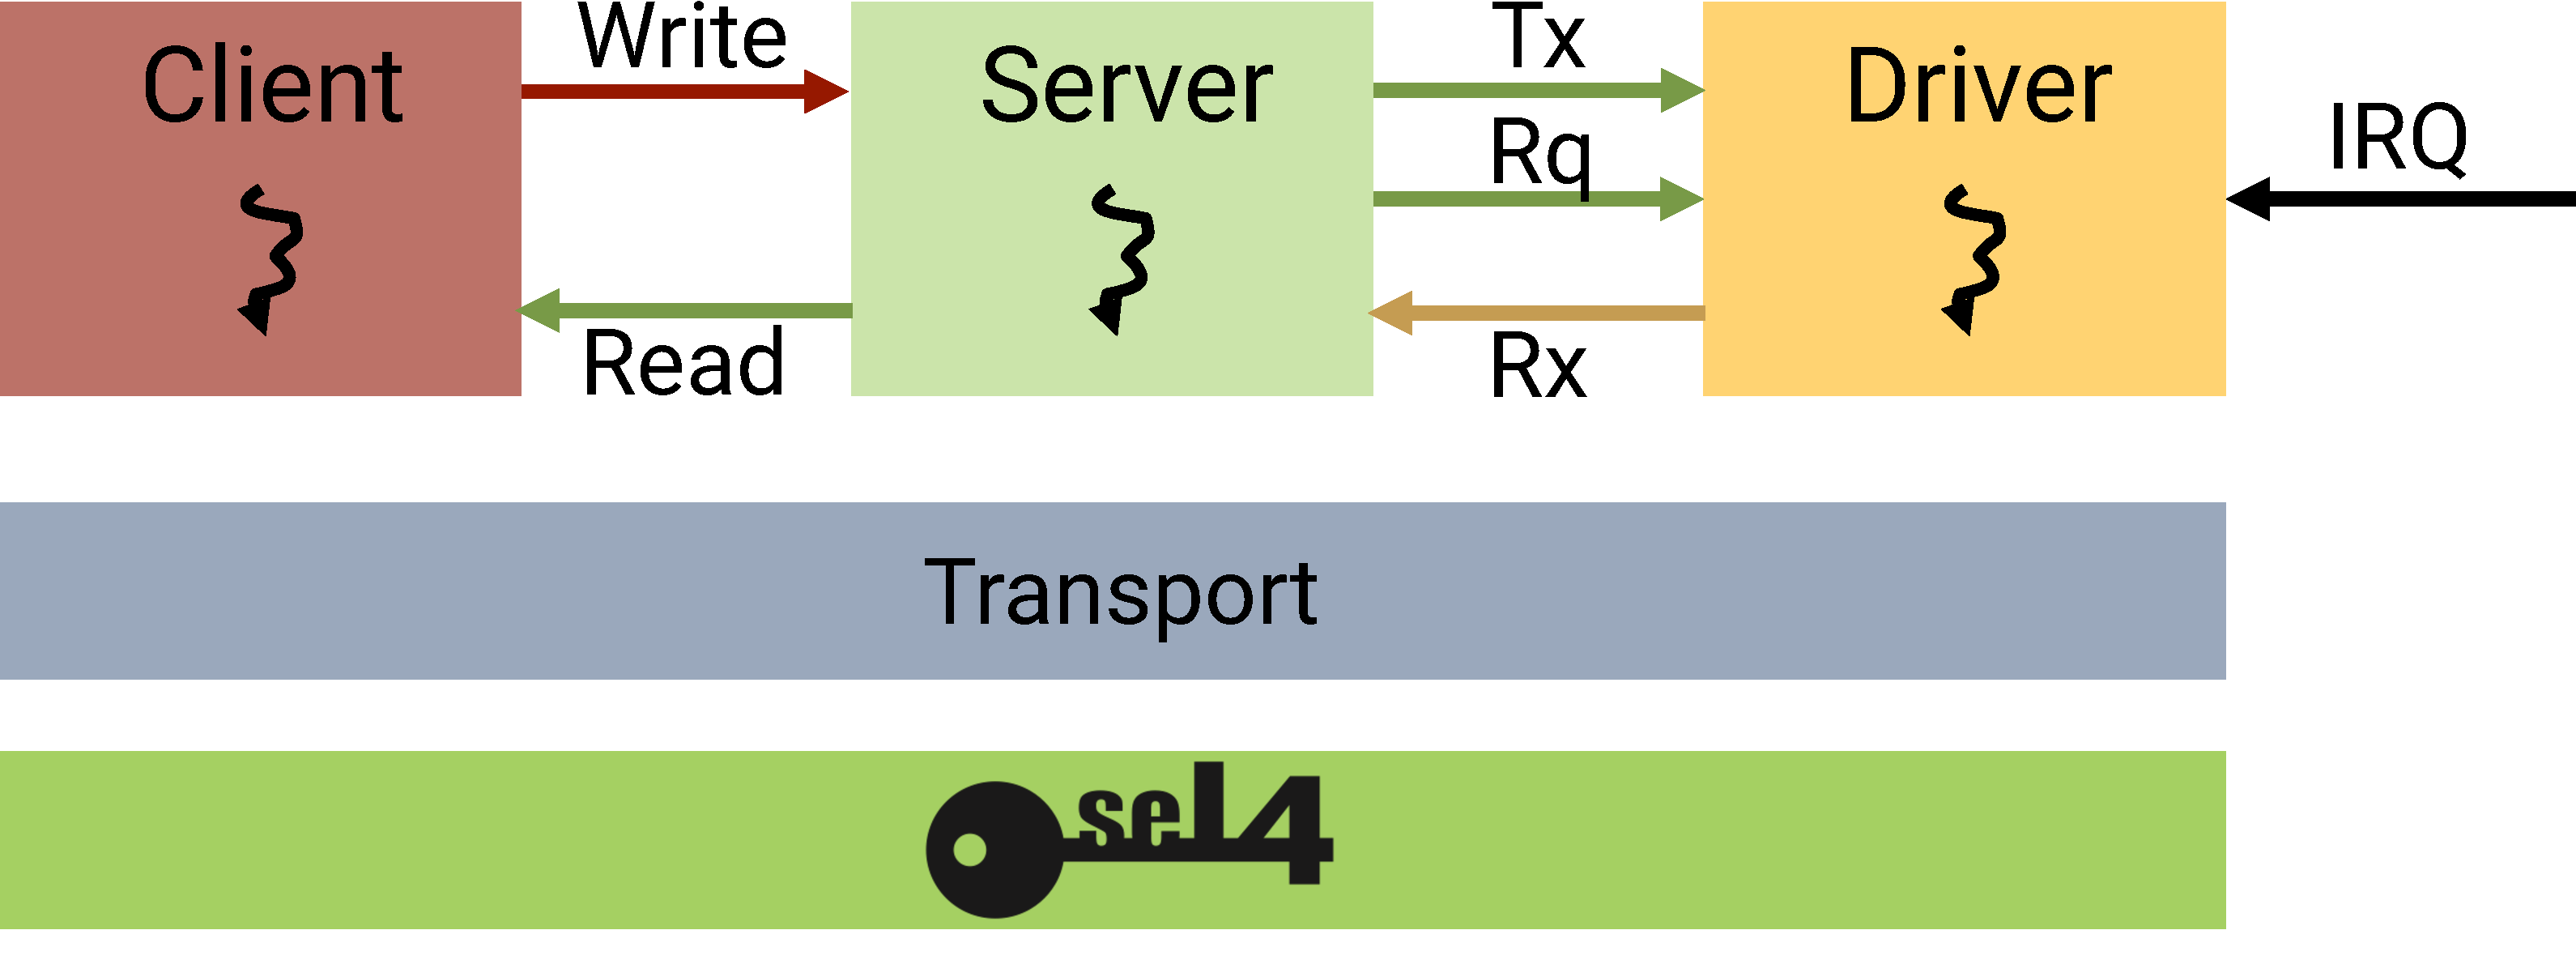
\includegraphics[width=9cm]{sddf.pdf}
    \caption{The seL4 Device Driver Framework (sDDF) \cite{Parker_22:sddf}}
    \label{f:sddf}
\end{figure}

The seL4 Device Driver Framework (sDDF) aims to rectify any performance degradation of a microkernel
design by providing interfaces and protocols to write performant yet secure user level device
drivers on seL4 \cite{Parker_22:sddf}. It currently supports a statically defined, minimal networking-focused system, and is 
developed on top of the seL4 microkit. The sDDF prioritises a strong separation of 
concerns by componentising each task in an I/O framework such that each component has only a 
single job. This keeps each component inherently very simple, not only minimising any debugging effort required by 
developers but also makes these components accessible to verification. The sDDF design is based on
top of a simple transport layer that provides protocols for communication between drivers and other
components in the system.

\section{Driver Model}\label{s:driver_model}
The device driver translates a hardware specific device protocol into a hardware independent
(but OS specific) device class protocol. It is inherently event driven, as it only needs to react to
either a client request or an interrupt generated by hardware, and in this way, it maps perfectly onto
the seL4 microkit model. Clients make requests through shared memory and seL4 asynchronous notifications
which simplifies the device driver code to an event loop reacting to either client requests or hardware
events as shown in \autoref{l:driver_pseudo}. 

\begin{figure} [H]
\begin{minted}[]{c}
main() {
    init()
    while(true)
        event = Wait()
        if (event & IRQ)
            handle_irq()
        if (event & CLIENT_REQ)
            handle_request()
}
\end{minted}
\caption{Driver pseudo code}
\label{l:driver_pseudo}
\end{figure}

\section{Transport Layer}
The sDDF transport layer consists of 3 distinct shared memory regions, data structures for data management
and access protocols. These memory regions are:
\begin{enumerate}
    \item \textbf{Metadata region}: the control registers of a device shared between the device itself and its driver. 
    This region is volatile as it is accessed directly by the device and is mapped uncached. 
    \item \textbf{Data region}: buffers containing data that's shared between the device and PDs that require access to the data.
    This region is also accessed directly by the device, but is mapped cached as we assume the device will only access it when 
    instructed. Before and after such accesses, we need to invalidate or clean buffers to ensure cache coherency.
    \item \textbf{Control region}: data structures to manage buffers in the data region. This is shared between two PDs in the system. 
\end{enumerate}

% Something about how we can just update these regions and issue notifications.
\subsection{Control region}
The control region consists of lockless ring buffer queues. These queues are single-producer,
single-consumer (SPSC) which keeps the implementation simple.
The queues keep track of addresses in the data region as shown in \autoref{f:control}. For simplicity,
the figure only shows the control region on the transmit path between a server and driver. Each pair of 
communicating PDs in the sDDF have their own shared control region but share the data region with other PDs. 
The sDDF uses two queues per direction, per control region. For example, as per \autoref{f:control}, the 
Transmit Used (TxU) queue stores buffer addresses which contain data ready for transmit. 
The Transmit Free (TxF) queue stores buffer addresses available for reuse. This is duplicated for the receive path.
The queues enable data to be passed between components in batches, thus minimising the number of system calls requried. 

\begin{figure}[h]
    \centering
    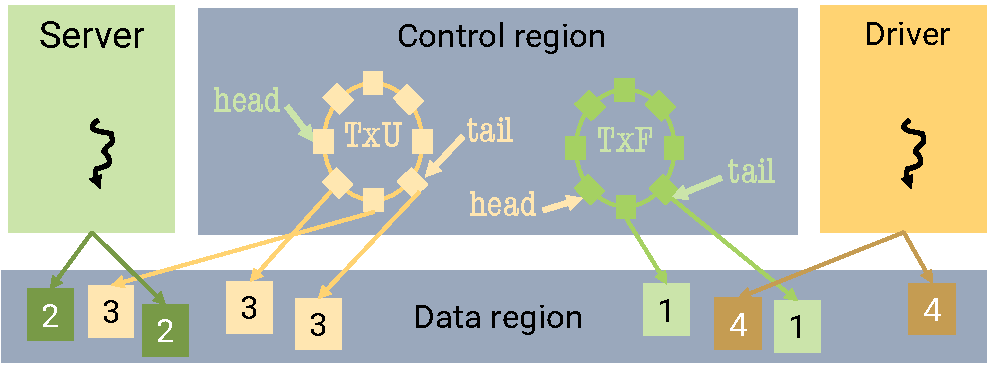
\includegraphics[width=12cm]{control_region.pdf}
    \caption{Control region between driver and server on transmit path \cite{Parker_22:sddf}}
    \label{f:control}
\end{figure}

The ring buffer queues themselves are very simple. \autoref{l:queues} shows the data structures. Each
ring buffer has a separate head and tail pointer, and entries between the tail and head point to a valid buffer
in the respective data region. Each ring buffer has exactly one producer (the server in \autoref{f:control})
and one consumer (the driver in \autoref{f:control}). The producer
only ever updates the head and the consumer only ever updates the tail.

\begin{figure} [H]
\begin{minted}[]{c}
struct buffer_descr {
    void   *address;
    size_t length;
}
struct ring_buffer {
    uint32_t head;
    uint32_t tail;
    struct buffer_descr buffer[RING_SIZE];
}
\end{minted}
\caption{Ring Buffer Queues}
\label{l:queues}
\end{figure}

Lock free updates to these queues are possible by utilising the property that reads and writes of small
integers are atomic. We simply use a \emph{write memory barrier} before updating the head or tail pointers
as shown in \autoref{l:queues2} to ensure that no reads or writes are re-ordered by the compiler or
processor across this point. As the code ensures there is at least one unused buffer between the head and tail,
the data race is benign and the memory barrier is sufficient to ensure consistency.

\begin{figure} [H]
\begin{minted}[]{c}
bool full(struct ring_buffer *ring)
{
    return (ring->head - ring->tail + 1) % RING_SIZE == 0;
}
bool empty(struct ring_buffer *ring)
{
    return (ring->head - ring->tail) % RING_SIZE == 0;
}
void enqueue(struct buffer_descr *buffer, 
            struct ring_buffer *ring) 
{
    assert ( !full(ring) );
    ring->buffer[ring->head % RING_SIZE] = *buffer;
    barrier();
    ring->head += 1;
}
struct buffer_descr *dequeue(struct ring_buffer *ring)
{
    struct buffer_descr *buffer;
    if (empty(ring)) {
        return NULL;
    } else {
        *buffer = ring->buffer[ring->tail % RING_SIZE];
        barrier();
        ring->tail += 1;
        return *buffer;
    }
}
\end{minted}
\caption{Ring Buffer Queue Management}
\label{l:queues2}
\end{figure}

\section{Device Sharing}\label{s:mux_design}
In order to share a device with potentially multiple client applications, the sDDF proposes a simple PD whose 
sole concern is multiplexing the hardware. This multiplexer is implemented at layer one, meaning each client application has its
own virtualised MAC address, and the multiplexer keeps a 1 to 1 mapping of MAC addresses and client CC ids. Multiplexing at layer two
or three would also be possible, but would mean confining applications to a particular protocol or set of ports. 
The multiplexer
can be separated into two separate components. One component handles incoming traffic (Rx Mux), and the other, outgoing traffic
(Tx Mux) as shown in \autoref{f:mux}. Control regions are used by each of these components to communicate with the component on 
either side.
In order to prevent clients from the ability to access each others' data, the shared data region must be split into
separate pools, and a simple copy component per client is responsible for copying data from one memory region to another.
\begin{enumerate}
\item \textbf{Shared Rx data region}: This data region is accessed directly by the device for writing newly received data, as well
as into the Rx Mux's address space and each of the copy components.
\item \textbf{Client Rx data regions}: This data region is mapped into a particular client's address space as well as this
client's copy component. There is a separate client Rx data region per client. The copy component copies data from the 
shared RX data region to the client's own Rx data region.
\item \textbf{Client Tx data regions}: This data region is accessed directly by the device to transmit data, but is also mapped into
the Tx Mux's address space and a particular client's address space. There is one client Tx data region per client. This
enables a zero copy interface on the transmit path.
\end{enumerate}

\begin{figure}[h]
    \centering
    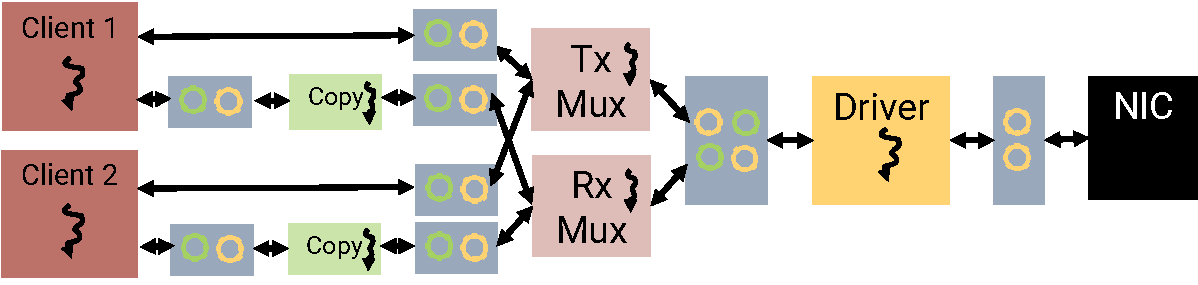
\includegraphics[width=\textwidth]{mux_design.pdf}
    \caption{Multiple client applications on the sDDF}
    \label{f:mux}
\end{figure}

A multiplexer servicing multiple components inherently requires a policy to determine the order in which it will process work,
however, the sDDF is currently limited to a signle client and as such, does not contain any policy at this stage. Furthermore,
a layer one multiplexer with multiple client applications requires special handling of broadcast protocols. 

\section{Control Flow}
Each component in the sDDF, aside from the client applications, is a single-threaded event-driven program. The
components are simply reacting to an update in either the control or metadata regions, signalled by an seL4 notification. 
To minimise the number of system calls, each component processes as many buffers as it can before signalling the next
relevant component.
The driver runs at the highest priority in the framework. This ensures timely handling of interrupts, as well
as immediate reaction to requests. In order to prevent the driver from monopolising the processor in the case
of high traffic on the receive path, we can limit the size of the receive queue in the metadata region and/or 
the size of the receive queues in the control regions.
The remaining priority ordering is as follows:

\centerline{Driver \(>\) Tx Mux \(>\) Rx Mux \(>\) Clients and per client copiers.}

This priority ordering enables components on the receive path to process as many packets as possible and
thus batch system calls. Due to the bounded size of the queues, only a limited number of packets 
can be processed in one invocation which provides flow control for lower priority components. Note that
client applications may have different priorities. In the case that client A has higher priority
than client B, then it may make sense that client B's copier has lower priority than that of client A.
However, to enable batching, clients should run at lower priority than their copy component. 
On the transmit path, components are invoked as soon as packets are 
ready to be transmitted which keeps transmit latencies low.

\subsection{Current Limitations}
The prototype, as of the start of this thesis, did not support multiple client applications and 
was limited to single core systems. As such, the multiplexer components were very simple and did not contain any policies. Furthermore, the 
design was limited as it expected a client application with symmetric traffic on the receive and transmit paths. In a real
networking system, this would not be the case. For example, a web server would have much higher throughput on the transmit path than the receive path.
Finally, all previous evaluations were limited to running on a single core only which is not the typical set up for high throughput networking systems.
% TODO: Add other stuff that is currently unsupported: eg device discovery, hot plugging, extension for virtual machines although this is out
% of scope for this thesis.

\section{Thesis Problem Statement}
This thesis addresses challenges in developing and evaluating a networking system based on 
the seL4 microkernel and the seL4 Device Driver Framework (sDDF). The overarching 
problem statement encompasses multiple key objectives. Firstly, the aim is to extend and evaluate 
the sDDF framework to provide flexible and secure support for multiple client applications, 
addressing diverse networking demands. Secondly, this thesis focuses on assessing the scalability 
of the framework to multi-core systems, investigating its efficiency across multiple cores to 
optimize performance in a multi-core environment. Additionally, this thesis aims to evaluate the 
framework's resilience against untrusted client applications, examining potential security vulnerabilities 
and proposing a simple solution to protect the subsystem in a given threat scenario from misbehaving clients. \\

These objectives collectively contribute to advancing microkernel-based networking systems, offering
a foundation for flexible, scalable, and secure support for multiple client applications while addressing
security concerns associated with untrusted clients. 


%\chapter{Approach}\label{ch:approach}
To achieve high performance I/O on seL4, this thesis will extend the current seL4 Device Driver Framework prototype 
to securely support multiple client applications on a multicore system. While doing so, 
we will evaluate the sDDF design while improving any bottlenecks in the current implementation
and optimise the system for large scale, high throughput networking systems.

\section{Design Goals}
When extending the sDDF, we wish to maintain the current prototype's design goals. 
Specifically, these are:
\begin{itemize}
\item \textbf{Radical Simplicity}: Each component in the framework should be kept as simple as possible. While verification is outside the scope
of this thesis, keeping each component simple will aid any future verification effort while assisting developers to reason about it.
\item \textbf{Strict separation of concerns}: Each component has one and only one job to do. 
\item \textbf{Swappable policy}: Any policy enforced by the framework should be swappable for another policy for different use cases.
This enables the framework to be flexible and support different use cases while keeping the implementation simple.
\item \textbf{Secure}: The framework should be secure by taking advantage of the security properties provided by seL4. seL4 guarantees
complete isolation of user-level components, and its capability system provides fine grained access control. This motivates the framework to apply
the principle of least authority: components \emph{only} have the minimum capabilities required to perform their job. Clients must not be able
to interfere with one another. 
\item \textbf{Performance}: The solution should be performance competitive with the current prototype (see \autoref{ch:sddf}),
as well as with other existing I/O frameworks (see \autoref{ch:related_work}).
\end{itemize}

\section{Methodology}
To accomplish our goal, we need to:
\begin{enumerate}
    \item Implement policies for the multiplexers, \autoref{s:mux_pol}
    \item Support broadcast protocols, \autoref{s:arp}
    \item Implement different client applications that imitate different use cases, \autoref{s:client}
    \item Add a second client to the prototype for testing, \autoref{s:client2}
    \item Support execution across multiple CPUs, \autoref{s:multicore}
    \item Perform a threat analysis of the framework to outline, and where possible, improve any
         security vulnerabilities in our design, \autoref{s:security}
    \item Evaluate and optimise: evaluate the solution by benchmarking the system throughout development 
    and improve any performance bottlenecks.
\end{enumerate}

\subsection{Multiplexer Policies} \label{s:mux_pol}
The current implementation is configured for a single client application. As such, neither the receive multiplexer
nor the transmit multiplexer contain any policy for handling multiple clients.\\
On the receive path, packets should be handed to the appropriate client on a first in, first out basis. However, 
in the case that a client cannot keep up with the incoming traffic and the client's received used (RxU) queue becomes full,
the multiplexer will start dropping packets. As the sDDF contains a single pool of shared buffers on the receive path,
a low priority client that cannot keep up with incoming traffic has the potential to starve a higher priority client, 
because there will be a shortage of free buffers for incoming packets. In order to prevent this, the system needs
to limit incoming throughput of lower priority clients by reducing the client's RxU queue size. The queue will 
fill up faster, and the multiplexer will drop packets earlier, which ensures a larger availability of shared buffers.\\
On the transmit path, the policy will depend on the particular use case as outlined in \autoref{s:mux_design}. Each of these
policies will need to be implemented with the design goals in mind.\\
Furthermore, the current transport layer does not track where buffers originated from. As each client has its own
pool of transmit buffers, the multiplexer needs to ensure the transmit buffer is returned to its origin after use.

\subsection{Support broadcast protocols}\label{s:arp}
The address resolution protocol (ARP) broadcasts packets to all applications in order to map a protocol
address (IPv4) with a MAC address. As the multiplexer will not know how to handle these packets/which client
to pass them on to, we could either develop a separate component to handle all broadcast traffic, or
alternatively, add the functionality to the MUX RX to duplicate these packets and forward them to all clients.
A separate component can be kept simple, as per the design goals with the aim of enabling eventual verification. It just
requires the necessary functionality extracted from an IP stack to respond to ARP. However, as ARP is based on both 
MAC address and protocol address, the ARP component would need to have a mapping of MAC address and
IPv4 address for each client. As each client could potentially alter
their IPv4 address, or change protocols altogether, this mapping would need to be done dynamically.\\ 
Alternatively, if we were to duplicate broadcast packets and forward them to all applications, the MUX RX would need to ensure
each client side receive free (RxF) queue was not empty in order to provide the MUX RX with enough free buffers to forward broadcast
packets. \\
Both designs need further evaluation to properly compare the trade-offs before we can support broadcast traffic.

\subsection{Imitate different client applications}\label{s:client}
The current implementation of the client application consists of a simple echo server. However, the client 
is limited as it expects to only ever transmit a packet after it has received one. This works for symmetric 
traffic, but does not test the system against clients with different networking demands. A webserver, for example, 
requires much higher throughput on the transmit path than the receive path. In order to mimic such a use case,
we want to design simple client applications with an event-driven model. This is because the client may need to
use more transmit buffers than are currently available in the transmit free queue. The client should then temporarily 
pause the current context while waiting for more free transmit buffers, so it is available to react to other events. 
Once more transmit free buffers are available (by which the client will be notified), the client can resume the transmit context. 
To support this, we must add continuations in the client application. This will enable us to easily imitate
different use cases with different networking demands when benchmarking.

\subsection{Add a second client to the prototype}\label{s:client2}
Adding another simple client application will be straight forward as we can re-use a lot of the code for the 
original single client application. Now there are two client applications, we want to thoroughly test the
framework to see if it performs as expected. Specifically, we want to experiment with the different 
policies developed in \autoref{s:mux_pol}, as well as different client demands. Such demands could be
symmetric traffic tested with a simple echo application as well as asymmetric traffic, tested with a client
application that either mostly receives packets but does not transmit frequently, or vice versa. Another variable
that would change the flow of the system would be experimenting with the clients' priorities. All up, we have the
following variables to experiment with:

\begin{itemize}
    \item Client priorities for scheduling. Either:
        \begin{enumerate}
            \item Client 1 runs at higher priority than client 2.
            \item Client 1 and client 2 have equal priority.
            \item Client 2 runs at higher priority than client 1.
        \end{enumerate}
    \item Client functionality. Each client could implement one of the following applications:
        \begin{enumerate}
            \item Echo application.
            \item Higher proportion of transmit. Eg. For every received packet, the client sends 100.
            \item Higher proportion of receive. Eg. For every 100 packets received, the client sends 1.
            \item Client initiated transmit. Client will transmit packets on a time out, regardless of the receive path. 
        \end{enumerate}
    \item Transmit Policy. This could be one of the following options:
        \begin{enumerate}
            \item Priority based. Client 1 takes higher priority over client 2. 
            \item Round robin. The multiplexer will alternate between responding to client 1, then client 2.
            \item Throughput based. Limit both clients' throughput to specified amounts. This could be 
            an even distribution or client 1 has a higher bandwidth limit to client 2.
        \end{enumerate}
    \item Receive flow control policy. If the clients themselves have equal priority, then this won't be necessary. 
    However, if they do not, then we can set the lower priority clients RxU queue size to a percentage of the
    higher priority client's queue size.
\end{itemize}

\subsection{Support multicore systems}\label{s:multicore}
The sDDF is implemented on top of seL4CP, which already supports multicore systems, so there are minimal changes required
to achieve this. As the transport layer is lock-free and system calls are kept to a minimum, the framework itself 
\emph{should} be capable of exploiting the parallelism of multicore hardware, by pinning components each to their 
own core. However, if there are not enough cores available, we require a policy to determine how components are distributed
across cores. For the prototype, a simple user level CPU utilisation analysis should reveal the most appropriate combinations.
This is achievable through seL4's benchmarking library.\\
Furthermore, it is possible to split the driver into two separate components. One component would be responsible for
handling client initiated events (predominantly transmit requests), while the other component would react to 
hardware events. This separation has the potential to achieve more performance on a multicore system as
each of these components could run concurrently on separate cores.\\
Additionally, concurrent execution could likely reveal bugs in the implementation or performance bottlenecks. Thorough 
analysis of results will be key in identifying this.

\subsection{Security Analysis}\label{s:security}
Component communication in the sDDF relies on shared memory and asynchronous notifications. While asynchronous communication
has considerable performance benefits (see \autoref{ch:related_work}), it means we trust each component to abide by the protocol. 
Future work, left out of scope of this thesis, will explore verifying all trusted components. However, this excludes the client
applications. We therefore must evaluate the client interfaces to ensure that a misbehaving client cannot interfere with other clients
nor any of the trusted components, including shared components such as the multiplexers. 

%\subsection{Port the sDDF to an x86 architecture with a 10Gbps NIC}\label{s:ixgbe}
%The current prototype runs on the Armv8 architecture. While this architecture is commonly used in IoT systems requiring
%high throughput networking, a significant portion
%of related work has been implemented and benchmarked on an x86 system. In particular, these systems use an ixgbe Ethernet
%driver. In keeping with our design goal of performance, having benchmarks on the same hardware as other high performance
%networking systems would allow us to better compare results.\\
%The seL4 Core Platform does not currently support x86 architectures, and nor do we have a working ixgbe driver for seL4. 
%Both of which are required for this goal.

\chapter{Design}\label{ch:design}

To achieve high performance I/O on seL4, this thesis will extend the current seL4 Device Driver Framework prototype 
to securely support multiple client applications on a multi-core system. While doing so, 
we will evaluate the sDDF design while improving any bottlenecks in the current implementation
and optimise the system for high performance networking systems.

When extending the sDDF, we wish to maintain the current prototype's design goals. 
Specifically, these are:
\begin{itemize}
\item \textbf{Radical Simplicity}: Each component in the framework should be kept as simple as possible. While verification is outside the scope
of this thesis, keeping each component simple will aid any future verification effort while assisting developers to reason about it.
\item \textbf{Strict separation of concerns}: Each component has one and only one job to do. 
\item \textbf{Swappable policy}: Any policy enforced by the framework should be swappable for another policy for different use cases.
This enables the framework to be flexible and support different use cases while keeping the implementation simple.
\item \textbf{Secure}: The framework should be secure by taking advantage of the security properties provided by seL4. seL4 guarantees
complete isolation of user-level components, and its capability system provides fine grained access control. Untrusted clients must not be able
to interfere with one another, nor any of the trusted shared components such as the multiplexers. 
\item \textbf{Performance}: The solution should be performance competitive with the current prototype,
as well as with other existing I/O frameworks (see \autoref{ch:related_work}).
\end{itemize}

To accomplish our goal, we need to:
\begin{enumerate}
    \item Implement policies for the multiplexers, \autoref{s:mux_pol}
    \item Support broadcast protocols, \autoref{s:arp}
    \item Support different client applications that imitate different use cases, \autoref{s:client_apps}
    \item Support execution across multiple CPUs, \autoref{s:multicore}
    \item Perform a threat analysis of the framework to outline, and where possible, improve any
         security vulnerabilities in our design, \autoref{s:security}
    \item Evaluate and optimise: evaluate the solution by benchmarking the system throughout development 
    and improve any performance bottlenecks.
\end{enumerate}

\section{Multiplexer Policy} \label{s:mux_pol}

A multiplexer servicing multiple components inherently requires a policy to
determine the order in which it will process work. Rather than designing a generic policy
that aims to cater to all possible use-cases, we instead
design several different multiplexers that implement a simple policy for a specific use-case. 

Both the Rx and Tx multiplexers are trusted components,
and thus are kept intentionally simple to leave them accessible to formal verification.
The main tasks of the multiplexers, regardless of policy implemented, are as follows:

\begin{itemize}
    \item Given a virtual address from the client/copier, translate it to a physical address before
            handing it over to the driver.
    \item Given a physical address from the driver, translate it to a virtual address before
            handing it over to the client/copier.
    \item Sanitise any buffer addresses from the client before forwarding them.
    \item Sanitise any addresses from the driver. 
    \item Transmit buffers belong to the client, and therefore all free buffers on the transmit path
            must be returned to the appropriate client.
    \item Receive buffers belong to the driver, and therefore all free buffers on the receive path
            must be returned to the driver.
\end{itemize}

%    \item The transmit multiplexer has the ability to sanitise the Ethernet header of outgoing packets
%to ensure the destination MAC address is well formed and will not cause issues
%on the network. Modern NICs are capable of sanitising headers of outgoing packets,
%%but many systems may require a design whereby the NIC is not trusted to perform this check 
%and thus it should be done in software.

\subsection{Receive Policy}\label{s:rx_policy}

All incoming packets are processed in FIFO order. The multiplexer contains a 
mapping of virtualised client MAC addresses and client queues. After dequeuing an incoming packet,
the multiplexer must first invalidate the cache (to ensure subsequent reads are fetched again from memory)
and read the packet header. The packet header contains the destination MAC address and if the packet is
addressed to a client on the system, the buffer address is forwarded to the appropriate client. 
If a client's Receive Used (RxU) queue is full, the multiplexer drops the packet and the buffer address is returned to
the driver. This can be prevented for higher priority clients by appropriate choice of client's RxU queue
sizes. Appropriate sizes can be selected based on experiments discussed in \autoref{ch:evaluation}.

The multiplexer must also return free buffers to the driver to be reused again. If a clients Receive Free
(RxF) queue is full, the multiplexer could stall the client while it waits to enqueue free buffers. Should this be the case,
the order in which the multiplexer processes the client RxF queue contains policy as it may
unblock clients. We propose instead to ensure the clients RxF queue is the same size as the number
of receive buffers circulating and thus prevent the client becoming blocked on waiting for this queue to be
processed. This design removes the need for policy on processing free buffers. \\ 

\subsection{Transmit Policy}

All incoming requests from clients are processed subject to a particular policy. 
We implement 3 different policies in \autoref{ch:implementation}:
\begin{enumerate}
    \item \textbf{Round robin}: whereby the multiplexer processes an outgoing request one at a time, alternating between clients.
    \item \textbf{Priority-based}: whereby the multiplexer prioritises client requests as per their given priority, processing as many
    requests as available for the highest priority client possible. 
    \item \textbf{Throughput-based}: whereby the multiplexer limits the available outgoing bandwidth per client at a time.
\end{enumerate}

The transmit multiplexer also returns
free buffers from the driver to the client in FIFO order, regardless of policy implemented on
processing transmit requests. However, the multiplexer has no way of knowing which client
a particular buffer belongs to before it has been dequeued. Should a particular client's 
Transmit Free (TxF) queue be full, the multiplexer could become blocked waiting to enqueue
a free buffer. We propose client TxF queues are at least 
the size of the number of buffers belonging to that client in order to prevent this. \\ 
Similarly, the drivers Transmit Used (TxU) queue should be at least the size of the sum of 
all client transmit buffers. This ensures the multiplexer will not become blocked on this queue
and thus disrupt the policy implemented to process client requests. \\ 

\subsection{Enforcing Policy Through System Design}
Depending on the greater system design, we expect some transmit policies to not work.
For example, given a single-core configuration, the higher priority multiplexer will
always be invoked as soon as a client has made a request to transmit. This means that
we can assume any other clients do not yet wish to transmit, or have not yet had the
opportunity to run to make a request. Therefore, the multiplexer does not need to 
consider all the client queues when invoked and can just service requests made
by the client that signalled. To enforce policy on multiple clients in such a scenario,
we rely on appropriate choices of client queue sizes and the scheduling parameters
of each client. For example, to enforce a round robin policy on two clients, we run both clients
at equal priorities, and limit their TxU queues to just one. This ensures
that each client will be stalled until their single request has been processed, and
another client will have the opportunity to run in the interim. The multiplexer will
then only process a single request per client at a time, though at the detriment to performance.\\
Similarly, should we require a priority based policy, we can assign appropriate priorities
to the clients scheduling parameters and limit lower priority client's queue sizes, thus relying on the scheduling
of the system to enforce this policy.\\
Finally, we can limit the client's queue sizes on both the transmit and/or receive paths
to limit the amount of either transmit and/or receive throughput available to each client.
Appropriate sizes can be selected based on experiments discussed in \autoref{ch:evaluation}.\\ 

\section{Broadcast Protocols}\label{s:arp}
Some protocols broadcast traffic to all systems by addressing the
Ethernet packet with a specific MAC address of ff:ff:ff:ff. However,
as the receive multiplexer is implemented at layer one and thus based on MAC addresses,
it will not know how to handle such packets. In particular, we need to support 
the Address Resolution Protocol (ARP), as it maps an
IPv4 address to a MAC address and thus 
is required for any network communication via Ethernet.\\
One possible solution is to copy these packets to all client applications.
This would require additional policy in the receive multiplexer that ensures
all client side RxF queues have enough free buffers available
for the multiplexer to dequeue and then copy broadcast packets into.
However, there are many different broadcast protocols, for example the Dynamic
Host Configuration Protocol (DHCP), and the arrival of such packets
can be nondeterministic. This makes it difficult to determine how many might arrive
simultaneously and thus how many buffers should be available in all client side
RxF queues at all times. If there are no any free buffers available for ARP, then
a client will not be able to receive any IPv4 traffic.\\
Instead, we implement a separate component to handle broadcast traffic. It interfaces
with the multiplexers the same as any other client, as shown in \autoref{f:arp}. 

\begin{figure}[h]
    \centering
    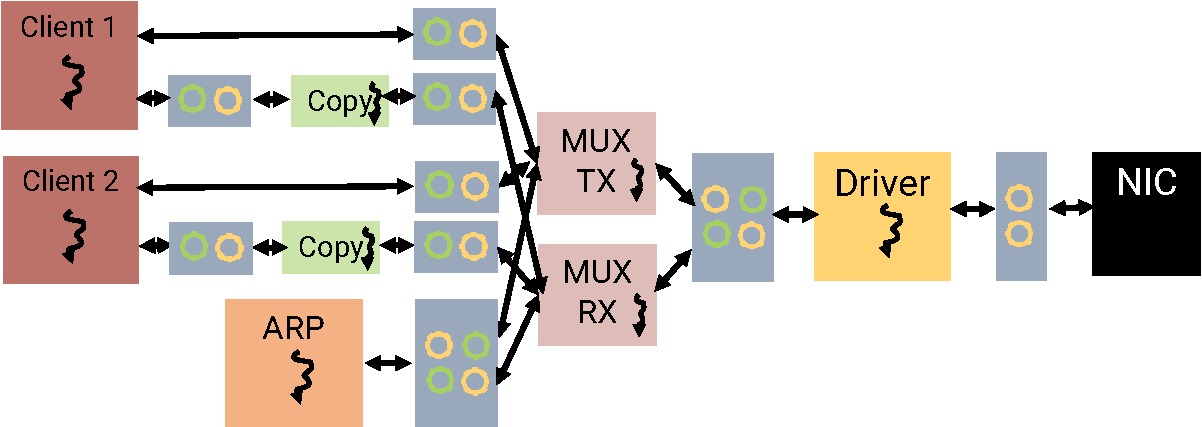
\includegraphics[width=\textwidth]{arp.pdf}
    \caption{Multiple client applications with an ARP component on the sDDF}
    \label{f:arp}
\end{figure}

\subsection{Separate ARP Component}\label{s:arp_design}
A separate ARP component only requires the minimal functionality to respond to 
the Address Resolution Protocol on behalf of any client applications running on
the system. In keeping with the design goals, this component will be kept 
very simple in the aims of enabling formal verification. Therefore we consider
this component to be trusted to maintain the integrity of its shared queues with
the multiplexer components as well as interfacing with clients and responding
correctly to ARP on behalf of the clients. \\
While supporting other broadcast protocols, such as DHCP, is out of scope of this thesis, 
the simplicity of the ARP component design enables its functionality to be extended easily
to support other broadcast protocols in the future. Such an extension would entail 
adding additional packet processing logic to our ARP component. 

\section{Client Applications}\label{s:client_apps}

The client application consists of a simple echo server and uses lwIP \cite{Dunkels_01} as an IP
stack library to process the network packet headers. The lwIP API stores packet data, including pointers
to the payload, in a \texttt{pbuf} struct. The \texttt{pbuf}s are allocated from static-sized memory pools and can be chained
together to produce a scatter-gather list.
On the receive path, \texttt{pbuf}s aren't chained together as the incoming payload already contains
all the required packet headers. However, when transmitting a packet via the UDP or TCP API, the \texttt{pbuf} will
only wrap around the actual payload, and in order to add the required headers, lwIP allocates additional \texttt{pbuf}s
containing these headers that are added to the head of a \texttt{pbuf} chain as shown in \autoref{f:pbuf0s}. \\

\begin{figure}[h]
    \centering
    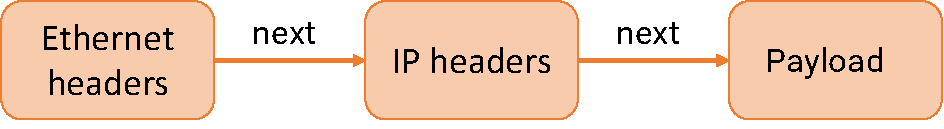
\includegraphics[width=0.6\textwidth]{pbufs0.pdf}
    \caption{Example lwIP \texttt{pbuf} list}
    \label{f:pbuf0s}
\end{figure}

Once a packet is ready to be transmitted,
a chain of \texttt{pbuf}s must then all be copied into a single sDDF buffer before being enqueued to the multiplexer.
The result of this design means that if there isn't a transmit buffer available for this chain of \texttt{pbuf}s, the
packet is dropped and the \texttt{pbuf}s are freed. While this is an acceptable outcome, it unfortunately means that a significant
amount of packet processing is then wasted. In order to combat this on the simple echo server and reduce
wasted cycles, packets are only
processed on the receive path depending on the availability of transmit buffers. This stalls the client application
until it receives a notification that more transmit buffers are available. \\

However, this solution is very limiting
as most networking applications do not have symmetric traffic. For example, a client application could receive a
higher number of packets than it transmits, and thus the design stalls the receive processing without reason. 
On the other hand, a client application with higher transmit demands would bypass the check for transmit buffers and result in
packets being dropped after packet processing. \\

To remove the premature check for transmit buffers on the receive path, we need to 
temporarily store the transmit context by storing the \texttt{pbuf} chains when there are not enough transmit buffers
available to the client. Once more transmit free buffers are available (by which the client will be notified),
the client can resume the transmit context. 

\begin{figure}[h]
    \centering
    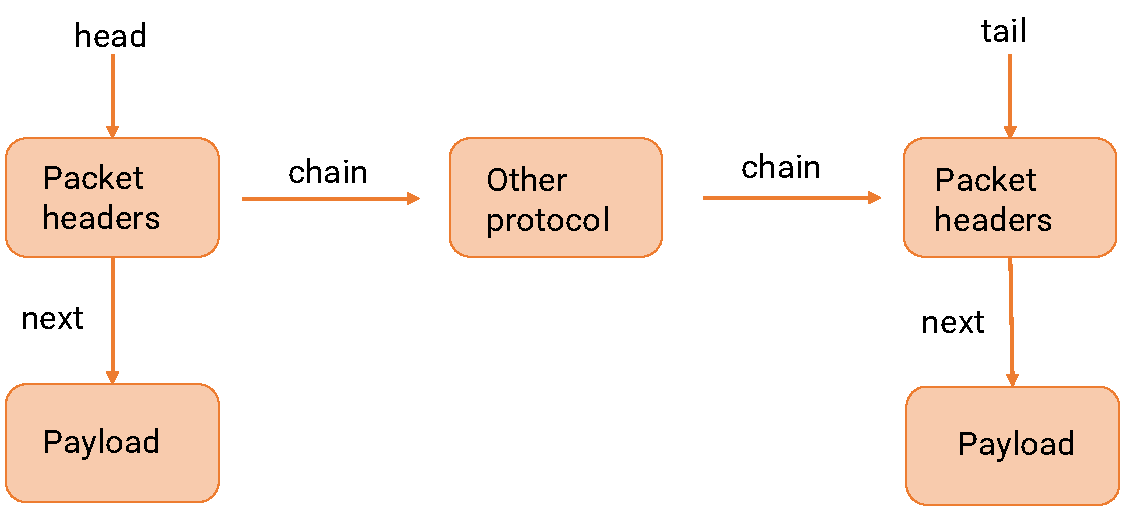
\includegraphics[width=0.7\textwidth]{pbufs.pdf}
    \caption{Example lwIP \texttt{pbuf} chain}
    \label{f:pbufs}
\end{figure}

We store the transmit context by simply linking \texttt{pbuf} chains together and storing the head and tail of the list. 
\autoref{f:pbufs} shows how multiple chains of \texttt{pbuf}s can be linked together. When a chain of pbufs is ready to
be transmitted, but there are not any free transmit buffers, we append the chain to the tail of the list and 
increment the reference count of the chain. This ensures the \texttt{pbuf}s won't be freed until they have actually been sent.
When a client is notified of the availability of more free transmit buffers, we dequeue \texttt{pbuf} chains from the head of
this list. This only requires adding a single extra field to lwIP \texttt{pbuf} structs. This simple change removes any
restriction on the receive path, sets up the client application to no longer expect symmetric traffic. We implement simple, example
applications with asymmetric traffic to evaluate how our framework copes with such loads in \autoref{ch:evaluation}.

\section{Multi-core Systems}\label{s:multicore}
The sDDF is implemented on top of the seL4 microkit, which already supports multicore systems
and so there are minimal changes required
to achieve this. As the transport layer is lock-free and system calls are kept to a minimum, the framework itself 
\emph{should} be capable of exploiting the parallelism of multicore hardware. We explore possible system designs in \autoref{ch:evaluation}.
Furthermore, it is possible to split the driver into two separate components. One component would be responsible for
handling client initiated events (predominantly transmit requests), while the other component would react to 
hardware events. This separation has the potential to achieve more performance on a multicore system as
each of these components could run concurrently on separate cores.\\

\subsection{Two-threaded driver on multi-core systems}
A device driver has multiple tasks: it must react to hardware events as signalled by an interrupt and it must react to software events,
such as a client request. Namely, the driver has 4 tasks:

\begin{enumerate}
    \item Dequeue incoming packets from the hardware receive ring and enqueue them to the RxU queue.
    \item Dequeue free buffers from the RxF queue and enqueue them to the hardware receive ring.
    \item Dequeue used transmit buffers from the TxU queue and enqueue them to the hardware transmit ring.
    \item Dequeue transmitted buffers from the hardware transmit ring and enqueue them to the TxF queue. 
\end{enumerate}

While these tasks involve interfacing with both hardware and software queues, each task involves
producing/consuming to different queues and reacting to different events. Task 3 occurs after a client transmit signal, 
tasks 1 and 4 occur after an interrupt, and task 2 occurs either preemptively after task 1 to ensure the hardware receive
ring is ready to be received, or after a client signal that more free buffers are available. We can split the driver up into
two separate components and simplify the workload as shown in \autoref{f:two_threaded_driver}.

\begin{figure}[h]
    \centering
    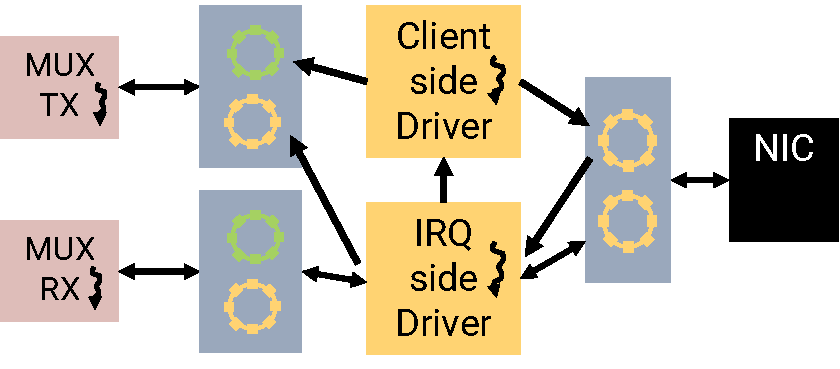
\includegraphics[width=0.6\textwidth]{two_threaded_driver.pdf}
    \caption{Driver architecture with two components}
    \label{f:two_threaded_driver}
\end{figure}

The client side driver is responsible for only task 3. It receives a signal from the transmit multiplexer when packets are ready
to be transmitted, and enqueues them to the tail of the hardware transmit ring. If the hardware transmit ring is full, it waits 
until it receives a notification from the IRQ side driver when space has freed up.\\
However, introducing an additional component to the framework will incur additional performance overheads due to extra context switches required.
We first analyse these overheads in \autoref{ch:evaluation} before concluding whether this design is appropriate on multi-core systems. 

\section{Security}\label{s:security}
Component communication in the sDDF relies on shared memory and asynchronous notifications. While asynchronous communication
has considerable performance benefits (see \autoref{ch:related_work}), it means we trust each component to abide by the protocol. 
Future work, left out of scope of this thesis, will explore verifying all trusted components. However, this excludes the client
applications. Our design should ensure a 
misbehaving client application does not have the ability to interfere with other clients and/or the rest of the system.\\

Clients receive data by dequeuing metadata, including buffer addresses, from a shared ring buffer, and transmit data by enqueuing such metadata. 
However, as these shared ring buffers are used by the components on either side of the client (e.g.. a multiplexer), we currently 
trust the client to maintain the integrity of the queues, and not write to buffers during DMA (i.e. once a packet has been enqueued
for transmit and before the buffer returns in the free queue). Specifically, we trust the client to:
\begin{enumerate}
    \item Update the tail pointer when dequeuing incoming packets from its RxU queue.\\
    While the rest of this queue can be mapped in as read only to the client, if the client does not correctly increment this pointer,
    the copy component will incorrectly see this queue as full/empty and potentially could either write over client's data or stop
    enqueuing new packets. As each client application has its own copy component, this potential vulnerability is isolated only to
    the misbehaving client.
    \item Write the correct metadata to the RxF queue once buffers can be recycled.\\ 
    Should a client not do this appropriately, for example, it could give a faulty buffer address/length, the copy component will not 
    use this buffer. This vulnerability is isolated to just the client and its copy component.
    \item Update the head pointer when enqueuing free buffers to its RxF queue.\\
    Like 2., this will only cause the copy component to not reuse newly enqueued buffers.
    \item Signal the copy component after enqueuing free buffers to its RxF queue.\\
    If the client does not inform the copy component of this update and the copy component is blocked on enqueuing incoming packets as there
    aren't enough free buffers to copy into, the copy component may not wake up. This could block any receive traffic to the misbehaving client
    but will not affect other components.\\
    Alternatively, if a client signals its copy component unnecessarily, this has the potential to increase networking latency. 
    As the copy component runs at higher priority than it's client, a signal from the client to its copy component will cause an immediate context
    switch. This has the potential to also affect other applications that run at equal or lower priority than the copy component on 
    the same CPU, as they may delayed to be scheduled as a result. seL4 already provides mechanisms to protect against such a scenario in 
    scheduling context objects. We can limit copy components' scheduling parameters such that they will not monopolise the CPU. Then, should 
    a client excessively signal its copier, the copy component will use up its scheduling budget and become blocked, thus reducing any Rx 
    bandwidth to that client. These limits
    will depend on greater system design, in particular, the scheduling parameters of all other applications running on the same CPU.
    \item No longer write data to buffers once enqueued to the clients RxF queue.\\
    Should the client write data to buffers already enqueued in the RxF queue, it will potentially write over incoming data. This will only
    affect the misbehaving client application, but can also be protected against by mapping Rx buffers to clients as read only.
    \item Enqueue a buffer to the RxF queue only once per use.\\
    If a client enqueues the same buffer multiple times to the RxF queue, it will potentially cause the copy component to write new incoming
    data over other used packets. This may mean the client loses Rx packets. Similarly, this will not affect any other applications.
    \item Write the correct metadata to the TxU queue.\\
    Should the client enqueue faulty metadata, such as a faulty address, the transmit multiplexer can detect this by ensuring the address lies inside
    that clients Tx DMA region, and will refuse this request without impacting any other components.
    \item Update the head pointer of the TxU queue.\\
    If the client does not correctly update this pointer, the multiplexer will not see newly enqueued packets and they may never be sent.
    \item No longer write to the packet after its enqueued to the TxU queue.\\
    Should the multiplexer be responsible for ensuring the packet is well formed with appropriate Ethernet headers, the client could potentially
    alter this data after sanitation and thus potentially send out corrupted packets. While modern NICs are typically equipped to prevent
    such errors, we don't want to always assume the device itself is trustworthy and corrupted packets have the potential to compromise
    other devices on the network.
    \item Signal the transmit multiplexer after enqueuing used transmit buffers.\\
    If the client does not signal the multiplexer, enqueued transmit packets may never be sent. This only affects the client itself.
    Alternatively, if the client signals the Tx multiplexer unnecessarily, it will increase latencies. Similarly to the receive path,
    a signal from client to Tx multiplexer causes an immediate context switch. Unnecessarily invoking the multiplexer will delay other 
    applications running on the same core at lower priority than the multiplexer.
    \item Update the tail pointer of the TxF queue after dequeuing free transmit buffers.\\
    If this is not done and the multiplexer incorrectly sees the queue as non empty, it may write over client data and
    thus potentially overwrite and therefore lose the clients transmit requests. If
    the multiplexer incorrectly sees the queue as full, it will panic. This is because the multiplexer assumes the client's 
    TxF queues are never full (as when it dequeues a new free buffer from the driver, it cannot know in advance where 
    to return the buffer). If one client misbehaves, then it may prevent the multiplexer from dequeuing more free buffers 
    from the driver side and returning them to clients. This has the potential the corrupt the entire transmit path for all
    client applications.
    \item Enqueue a buffer to the TxU queue only once per use.\\
    If a client enqueues the same buffer multiple times to the TxU queue, it will potentially cause the device to send the
    packet multiple times. This may affect lower priority clients by monopolising the device. An appropriate choice of Tx multiplexer
    policy can protect against this consequence, and thus only affecting the misbehaving client.
    \item Keep track of all buffers.\\
    Rx and Tx buffers belong to clients and it is up to the client to not lose buffer pointers. However, should a client lose
    buffers, it could potentially limit that clients available throughput. Clients do not have access to shared buffers so this
    will not affect any other clients.
\end{enumerate}

From the above analysis, and assuming all components other than the client applications are trustworthy,
we can conclude the receive path is secure. A trusted component, the copier, sits between the untrusted client application
and the shared multiplexer, and in each potential vulnerability whereby the client does not abide by the protocol, the copy component
will not enqueue/dequeue more incoming packets and thus starve only the misbehaving client. This assumes the RxU queue between 
the receive multiplexer and copy component is appropriately sized. Should this queue size exceed the number of shared buffers
available for all clients, and a client misbehaves, it could potentially starve other clients. This is because the copier
of a misbehaving client will not enqueue more incoming packets to the client (either temporarily or permanently), and the RxU queue
to the copier could then fill up. If there are limited shared buffers available and a high proportion are enqueued to the copier
of a faulty client, there will be less buffers available for other clients. To prevent such a scenario, we ensure there are enough
shared buffers on the receive path for all RxU queues between the multiplexer and each copy component to be full at the same time.\\

However, the transmit path is not protected from misbehaving client applications. While scenarios 7, 8 and 13 only impact the client
itself, scenario 7 has the potential to compromise other devices on the network without a trusted device, and scenario 9 can block
all transmit traffic, including that of other clients.\\

\subsection{Transmit Copy Component}

To remove these vulnerabilities, we can mimic the receive path by injecting a small, trusted component in between each untrusted
client application and the shared multiplexer as shown in \autoref{f:tx_copy}. The component can be configured as
per the system design, or even removed all together, as required by the threat scenario.

\begin{figure}[h]
    \centering
    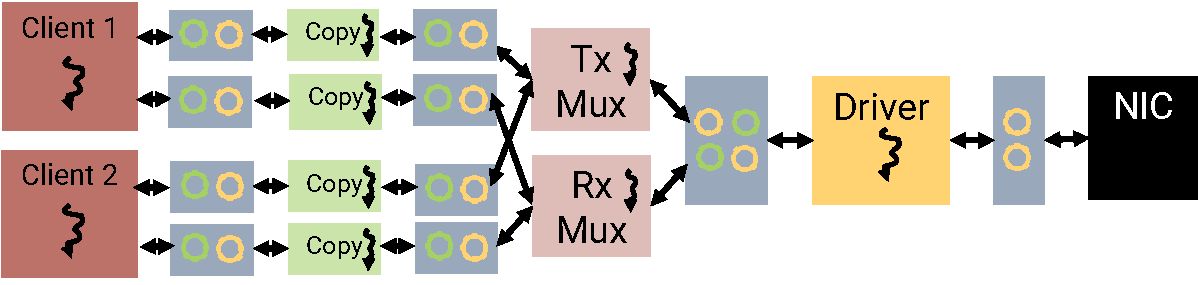
\includegraphics[width=\textwidth]{tx_copy.pdf}
    \caption{Architecture with an additional transmit copy component}
    \label{f:tx_copy}
\end{figure}

To interface with a completely untrusted client application, this new component needs to:
\begin{itemize}
    \item Ensure metadata enqueued to the multiplexer is sane.
    \item If the device is untrusted, check outgoing packets are well-formed and copy them into a separate region not mapped
          into the clients address space.
    \item Interface with the multiplexer correctly by incrementing the head/tail pointers as required.
    \item Ignore any transmit packets that do not abide by the protocols outlined above.
\end{itemize}

Like the receive path copy components, should a client misbehave when interacting with the shared queues, or fail to signal as per
the protocol, the new Tx Copy component will ignore any requests or no longer enqueue free buffers to the client, thus only disturbing
that client and not affecting any other components in the system.\\
This additional component would introduce some additional performance overheads. These include the cost of reading packet headers, 
an extra system call on the transmit path, and potentially the cost of copying the entire packet. 
We measure these overheads in \autoref{ch:evaluation}.\\

\chapter{Implementation}\label{ch:implementation}

Prior to this thesis, the seL4 Device Driver Framework already supported a minimal, single client
networking system. This included an Ethernet driver, layer-one Rx multiplexer (limited to a single 
client), copy component, a Tx multiplexer (also limited to a single client and containing no policy) and 
a simple echo server client application. To properly support multiple client applications, we
extend the Rx multiplexer to multiplex to multiple different client applications, and implement 3
new transmit multiplexers. We also implement a simple timer driver to interface with our 
transmit multiplexer when required, and finally, a new ARP component to handle broadcast traffic. 
We configure all queues between these components to further implement different
policies in \autoref{ch:evaluation}.


\section{Transmit Multiplexer Policies}

We implement 3 different transmit multiplexers, each implementing a different policy. 
We present our pseudo code designs for how each multiplexer process transmit packets from
the client. All multiplexers return free buffers from the driver to their respective 
clients in the same FIFO order and hence this function has been omitted for brevity. 

\subsection{Round Robin Policy}
We implement a round robin policy by processing a single client's transmit request at a time.
This is done in a loop to ensure we process any batched requests as outlined in \autoref{l:roundrobin}.

\begin{figure} [H]
    \begin{minted}[fontsize=\small]{c}
void process_transmit_ready() {
  enqueued = 0;
  old_enqueued = 0;

  while(!ring_full(driver->used_ring)) {
    old_enqueued = enqueued;
    for each client {
      /* Process a single used buffer at a time */
      if (!ring_empty(client->used_ring) &&
          !ring_full(driver->used_ring)) {
        
        buf = dequeue(client->used_ring);
        phys = get_phys_addr(buf);
        enqueue(driver->used_ring, phys);
        enqueued += 1;
      }
    }
      /* we haven't processed any packets since 
        last loop, exit */
    if (old_enqueued == enqueued) break;
  }
}
\end{minted}
\caption{Transmit Round Robin Policy}
\label{l:roundrobin}
\end{figure}

\subsection{Priority-based Policy}

We implement a priority-based policy in \autoref{l:prioritybased}. We assume the list of
clients is ordered from highest priority to lowest. Thus it is possible to change a clients
priority at run time by manipulating this list.\\

\begin{figure} [H]
    \begin{minted}[fontsize=\small]{c}
void process_transmit_ready() {
  enqueued = 0;
  old_enqueued = 0;
  while(!ring_full(driver->used_ring)) {
    old_enqueued = enqueued;
    for each client {
      while(!ring_empty(client->used_ring) &&
            !ring_full(driver->used_ring)) {

        buf = dequeue(client->used_ring);
        phys = get_phys_addr(buf);
        enqueue(driver->used_ring, phys);

        enqueued += 1;
        /* if a higher priority client has since 
            made a request, go again */
        if (!any_ring_empty(clients[:client])) break;
      }
    }

    if (old_enqueued == new_enqueued) break;
  }
}
\end{minted}
\caption{Transmit Priority-based Policy}
\label{l:prioritybased}
\end{figure}

\subsection{Bandwidth Limited Policy}\label{s:bandwidth}

We implement a bandwidth-limited policy in \autoref{l:bandwidth}. The multiplexer will 
process client transmit requests, calculating how much bandwidth the client has used based on
each request size in a given time window. Should a client exceed its limit within the time window,
the multiplexer will request a time out from the timer driver for the remaining time. As the multiplexer must
regularly communicate with the timer driver to get the time and set timeouts, we design a simple timer driver
API as shown in \autoref{l:timer}. 

\begin{figure} [H]
    \begin{minted}[fontsize=\small]{c}
void process_transmit_ready() {
  curr_time = get_time();
  for each client {
    if (curr_time - client->last >= TIME_WNDW) {
      client->last = curr_time;
      client->bandwidth = 0;
    }
    
    while (!ring_empty(client->used_ring) && 
           !ring_full(driver->used_ring) && 
           client->bandwidth < client->max) {

      buf = dequeue(client->used_ring);
      phys = get_phys_addr(buf);
      enqueue(driver->used_ring, phys);
      /* recalculate the clients bandwidth used in 
        the current time period */ 
      client->bandwidth = calculate_bandwidth(buf_size);
    }

    if (!ring_empty(client->used_ring) && !client->timeout) {
      set_timeout(TIME_WNDW - curr_time - client->last);
      client->timeout = true;
    }
  }
}
\end{minted}
\caption{Transmit Bandwidth Limited Policy}
\label{l:bandwidth}
\end{figure}

\begin{figure} [H]
    \begin{minted}[fontsize=\small]{c}
uint64_t get_time() {
  microkit_ppcall(TIMER, microkit_msginfo_new(GET_TIME, 0));
  return microkit_mr_get(0);
}
        
void set_timeout(uint64_t micros) {
  microkit_mr_set(0, micros);
  microkit_ppcall(TIMER, microkit_msginfo_new(SET_TIMEOUT, 1));
}
\end{minted}
\caption{Timer Driver API}
\label{l:timer}
\end{figure}

The timer driver is a high priority, passive server. It receives interrupts from the device,
and forwards these by notifying the appropriate client or multiplexer. The bandwidth limited
multiplexer reacts to such notifications by clearing the appropriate clients timeout and
recalling process\_transmit\_ready. Note that this implementation could be made more efficient
by mapping the timer registers read-only into the multiplexer's address space. This would remove
the need for a frequent system call to get the time. However, these implementations are 
meant only as example prototype rather than a prescribed implementation and further optimisations
have been left for use-case specific implementations. \\

This bandwidth-limited policy can also be combined with the round robin or priority based policy
to order each clients requests. Such a case would be useful in reducing the 
transmit latencies of latency sensitive applications.\\ 


\section{ARP Component}

We implement a separate ARP component that is responsible for handling all broadcast traffic. 
As client MAC addresses are assigned at system design time, our ARP component has a static
mapping of client IDs to virtualised MAC addresses. For client IDs, we use the clients 
communication channel ID as assigned by microkit. 

\subsection{Client Interface}
As ARP is based on both MAC addresses and IPv4 addresses, the new component
requires an interface with client applications. This interface will allow clients
to register a new IPv4 address, change an IPv4 address, or remove one. As adding,
changing and removing an IPv4 address is typically very infrequent for networking systems
and requires minimal data exchange, we define this interface using a protected procedure
call (PPC) from the client to the ARP component. The ARP component can use both the
client ID and the MAC address provided in the arguments to store the clients IPv4 address. 

\begin{figure} [H]
    \begin{minted}[fontsize=\small]{c}
void register_ip4(new_ip4_addr, mac_addr[6])
{
  /* split the MAC address across two registers so it fits */
  microkit_mr_set(0, mac_addr[0:4]);
  microkit_mr_set(1, mac_addr[4:6]);
  microkit_mr_set(2, new_ip4_addr);
  microkit_ppcall(ARP, microkit_msginfo_new(REGISTER_IP, 3));
}

void change_ip4(old_ip4_addr, new_ip4_addr, mac_addr[6])
{
  microkit_mr_set(0, mac_addr[0:4]);
  microkit_mr_set(1, mac_addr[4:6]);
  microkit_mr_set(2, old_ip4_addr);
  microkit_mr_set(3, new_ip4_addr);
  microkit_ppcall(ARP, microkit_msginfo_new(CHANGE_IP, 4));
}  

void remove_ip4(old_ip4_addr, mac_addr[6])
{
  microkit_mr_set(0, mac_addr[0:4]);
  microkit_mr_set(1, mac_addr[4:6]);
  microkit_mr_set(2, old_ip4_addr);
  microkit_ppcall(ARP, microkit_msginfo_new(REMOVE_IP, 3));
}
\end{minted}
\caption{Client Interface to ARP Component}
\label{l:arpintf}
\end{figure}

Currently, the ARP component can only store a single IPv4 address per client, which
is enough for our testing purposes, however this limit can be extended easily in the code
base should the need arise.\\

\chapter{Evaluation}\label{ch:evaluation}

% All policies implemented

% Multicore analysis, including user and kernel space cycles to show the overhead. 

% 
\chapter{Conclusion and Future Work}\label{ch:conclusion}

%% chapters in the ``backmatter'' section do not have chapter numbering
%% text in the ``backmatter'' is single spaced
\backmatter
\bibliographystyle{apalike}
\bibliography{pubs}

\end{document}
